\documentclass[letterpaper,twocolumn,10pt]{article}
% Preamble
\usepackage{booktabs}
\usepackage{tabularx}
\usepackage{array}
\usepackage{makecell}
\usepackage{usenix,epsfig}
\usepackage{amsmath}
\usepackage{booktabs}
\usepackage{makecell}
\usepackage[ruled,vlined,linesnumbered]{algorithm2e}
\setlength{\textfloatsep}{10pt plus 2pt minus 2pt}
\usepackage{tabularx}
\usepackage{xcolor}

% Pseudocode style: match the GMAX/NSDI look in Fig. 2.
% - ruled caption and bottom rule
% - line numbers
% - vlined L-shaped block guides (no explicit end-function/end-if text)
% - purple // comments, with no triangle marker
\definecolor{RavelCommentPurple}{RGB}{190,0,140}
\newcommand{\RavelComment}[1]{\textcolor{RavelCommentPurple}{#1}}
\SetCommentSty{RavelComment}
\SetAlgoNlRelativeSize{-1}
\SetNlSty{bfseries}{}{}
\SetKwProg{Fn}{Function}{:}{}
\SetKw{Return}{return}
\DontPrintSemicolon

\begin{document}
%don't want date printed
\date{}

%make title bold and 14 pt font (Latex default is non-bold, 16 pt)
\title{\Large \bf RAVEL: Reversible SLO-Aware Virtual Placement for Geo-Distributed LLM Serving}

% \author{
% {\rm Your N.\ Here}\\
% Your Institution
% \and
% {\rm Second Name}\\
% Second Institution
% }

\maketitle

% Use the following at camera-ready time to suppress page numbers.
% Comment it out when you first submit the paper for review.
\thispagestyle{empty}
\subsection*{Abstract}

Geo-distributed LLM serving pools GPU capacity across regions, but WAN
latency and heterogeneous SLOs make the \emph{value} of regional capacity
request-dependent: a region that is optional for one request may be the only
SLO-feasible choice for another. Committing placement immediately preserves
SLO slack but acts on incomplete demand information, whereas waiting to
observe subsequent arrivals consumes the very slack needed to meet the SLO.

We present RAVEL, an SLO-aware serving system that separates when demand
becomes visible from when placement becomes final. RAVEL tentatively assigns
each request to a serving replica and immediately attributes its prospective
demand there, while keeping the assignment revisable until successful engine
handoff. Subsequent arrivals can therefore redirect still-router-owned work
when scarce capacity is needed by more region-constrained requests. Because
reassignment ends at handoff, RAVEL requires no migration of engine-managed
KV state.

We implement RAVEL on vLLM across three geo-distributed clusters connected by
physical WAN paths. Across conversational, bursty, and completion-oriented
workloads, RAVEL consistently improves request-level SLO attainment as
offered load increases. At 16$\times$ load, RAVEL improves request-level SLO attainment over the
best-SLO baseline by 8.8, 11.2, and 16.6 percentage points on LMSYS, Burst,
and DeepResearch, respectively, while reducing P95 TTFT by 21.8--69.2\%
and P95 end-to-end latency by 14.7--34.5\%.

\section{Introduction}
\label{sec:introduction}

Geo-distributed LLM serving expands available GPU capacity, but not every
region is equally useful to every request.
Large-scale private WANs expose heterogeneous inter-region paths
~\cite{b4,swan}, while distributed inference systems must additionally
contend with heterogeneous accelerator, serving, and network conditions
~\cite{helix,cassini,skylb,gorgo,solyx}.
Together with heterogeneous request-level SLOs, these differences make
regional capacity request-dependent: a region that is merely attractive for
one request may be the only SLO-feasible choice for another.
A placement therefore determines not only GPU load and cache locality, but
also the WAN path and remote serving conditions experienced by the request.
Interactive requests may impose tight time-to-first-token (TTFT) and
time-between-token (TBT) bounds, whereas longer-running or multi-stage
requests may instead be governed by end-to-end completion or
quality-of-experience objectives
~\cite{distserve,jitserve,quartz,andes,revisit_slo_goodput}.
Consequently, allocating regional capacity well requires reasoning about both
current serving conditions and the SLO-feasible alternatives available to
each request.

Existing distributed routers improve \emph{where} an arriving request should
execute using signals such as serving load, cache locality, WAN conditions,
request-level SLOs, and adaptive routing feedback
~\cite{preble,dualmap,skylb,gorgo,quartz,lodestar}.
However, these routing abstractions largely couple destination selection with
commitment: once a request is assigned using the currently visible state,
later arrivals generally do not influence that placement before execution
begins.
This coupling creates an additional online allocation problem.
A locally attractive placement for the current request can consume
SLO-feasible capacity that a later, more region-constrained request cannot
replace.
The missing question is therefore not only
\emph{where should this request execute?}, but also
\emph{when should an earlier placement become irreversible?}

A two-request example shows why early commitment can waste SLO-feasible
capacity.
Consider two serving regions, $A$ and $B$.
The first request, $r_1$, can satisfy its SLO in either region, whereas a
later request, $r_2$, can succeed only in $A$.
When $r_1$ arrives first, $A$ may appear faster and therefore be selected by a
locally optimal router.
If $r_2$ arrives shortly afterward, however, this decision has consumed its
only feasible capacity.
Placing $r_1$ in $B$ instead would allow both requests to succeed:
\emph{region $A$ is merely faster for $r_1$, but it is essential for $r_2$}.
Thus, optimizing requests independently can reduce aggregate request-level
SLO attainment even when each individual placement appears reasonable when
it is made.

Delaying commitment can reveal the second request, but observation consumes
the same SLO slack needed for WAN transfer, queueing, and inference.
A fixed-delay late-binding policy can therefore observe more demand before
placing a request, yet every millisecond of added deferral also reduces the
time remaining to satisfy that request's SLO.
We call this tension the \emph{information--slack tradeoff}.
Figure~\ref{fig:motivation} illustrates it empirically:
a short fixed deferral can expose useful arrivals and improve SLO attainment,
but the benefit saturates as the deferral consumes an increasing fraction of
request SLO budgets.
This leaves a design opportunity between immediate one-shot placement and
fixed-delay late binding: make arrived demand visible immediately while
preserving only bounded, request-specific placement revisability.

RAVEL's key insight is that deferred commitment does not require deferred
accounting.
Rather than treating placement as one atomic decision, RAVEL separates when a
request begins influencing capacity planning from when its destination becomes
final.
On arrival, RAVEL obtains replica-specific SLO quotes, selects a tentative
serving replica, and immediately attributes the request's prospective demand
to that replica.
Later arrivals therefore observe earlier demand even while the corresponding
placements remain revisable.
While an eligible request remains Router-owned, newly revealed demand may
trigger bounded replanning and transfer both its tentative ownership and
prospective charge to another replica.
The placement becomes final only after successful engine handoff.
By stopping reassignment at this explicit boundary, RAVEL preserves
pre-handoff flexibility without migrating engine-managed KV state.

Realizing this separation safely and efficiently requires three capabilities.
First, RAVEL must determine which replicas remain SLO-feasible under
heterogeneous WAN delays, engine backlog, Prefill and Decode interference, and
request-specific success criteria.
It addresses this challenge with calibrated, replica-specific SLO quotes
derived from live serving state.
Second, tentative work must affect subsequent decisions without becoming
double-counted or stale after reassignment.
RAVEL therefore maintains transferable prospective accounting whose ownership
and replica-dependent charges move atomically with each tentative placement.
Third, revisability must not require repeatedly optimizing over every
outstanding request or delaying work indefinitely.
RAVEL restricts expensive replanning to a bounded Router-owned cohort and ends
all placement revision at the engine-handoff boundary.
Together, these mechanisms retain useful online flexibility while bounding the
latency and state-management costs introduced by the control plane.

We implement RAVEL as an asynchronous routing layer for
vLLM~\cite{vllm} and evaluate it using five serving replicas across three
clusters connected by physical WAN paths.
Our experiments cover conversational traffic, bursty arrivals, and
completion-oriented demand over six offered-load levels.
At $16\times$ load, RAVEL improves request-level SLO attainment over DualMap
by \textbf{8.8}, \textbf{11.2}, and
\textbf{13.4 percentage points} on LMSYS, Burst, and DeepResearch,
respectively.
At the same load, it reduces P95 TTFT by
\textbf{49.1--80.5\%} relative to DualMap.
The online replanning path remains millisecond-scale, with a measured P95
scheduling-pass latency of 2.10\,ms at Burst $12\times$ load.

In summary, this paper makes three contributions:
\begin{itemize}
    \item
    We identify the \emph{request-dependent value of regional capacity} and
    the resulting \emph{information--slack tradeoff}: committing too early
    ignores demand revealed by later arrivals, whereas waiting too long
    consumes the SLO slack needed for successful execution.

    \item
    We introduce an \emph{immediate-accounting, deferred-commitment}
    abstraction and realize it through replica-specific SLO quotes,
    transferable prospective accounting, bounded pre-handoff replanning, and
    an explicit engine-handoff commitment boundary.

    \item
    We implement RAVEL on vLLM and evaluate it on a physical-WAN deployment,
    demonstrating consistent SLO-attainment improvements across
    conversational, bursty, and completion-oriented workloads while retaining
    millisecond-scale online planning overhead.
\end{itemize}





\section{Problem and Design Opportunity}
\label{sec:problem}

The design opportunity arises from separating three decisions that request
routing often couples: \emph{placement}, \emph{regional demand accounting},
and \emph{commitment}.
A placement associates a request with a candidate serving replica and,
therefore, with the region containing that replica.
Regional demand accounting attributes an arrived request's prospective work
to its tentative replica and region so that the request influences subsequent
placement decisions.
Commitment is the boundary after which the routing layer no longer revises
that placement.
Using only causally available information, the router seeks to maximize the
fraction of requests that satisfy all applicable request-level SLOs.
RAVEL chooses successful handoff to the serving engine as its commitment
boundary: a request remains reassignable while it is Router-owned and becomes
final only after handoff.
This is a deliberate control-plane boundary rather than an inherent
irreversibility property of LLM execution; it preserves placement flexibility
without requiring migration of engine-managed KV state.



\subsection{Request-Dependent Regional Feasibility}
\label{sec:problem:feasibility}

Prior SLO-aware serving systems show that whether a request can meet its
latency objective depends on both request-specific requirements and evolving
serving conditions~\cite{distserve,jitserve,quartz,andes}.
RAVEL makes this dependence explicit at the geographic placement layer:
SLO feasibility is specific to a request, candidate replica, and decision
time rather than a static property of a region.

Let $c$ denote a serving region, $\mathcal{R}_c$ the replicas in that region,
and $r\in\mathcal{R}_c$ a candidate replica.
For request $i$, let $\Phi_{i,r}(t)$ indicate whether replica $r$ is predicted,
using only information available at time $t$, to satisfy every SLO constraint
applicable to $i$.
This prediction depends on the request's SLO semantics and remaining slack,
its estimated service demand, the WAN path to region $c$, and the currently
observed serving state at replica $r$.
Because both serving state and remaining slack evolve over time,
$\Phi_{i,r}(t)$ is an online feasibility estimate rather than a guarantee:
future arrivals and prediction error may still change the realized outcome.
Section~\ref{sec:design:feasibility} describes how RAVEL constructs these
replica-level predictions.

We define the feasible-region set of request $i$ as
\begin{equation}
    \mathcal{F}_i(t)
    =
    \left\{
        c
        \;\middle|\;
        \exists r\in\mathcal{R}_c:
        \Phi_{i,r}(t)=1
    \right\}.
    \label{eq:problem:feasible-set}
\end{equation}
The time index captures two distinct sources of change.
First, new arrivals and accounting updates alter the serving state visible to
the router, so $\mathcal{F}_i(t)$ may expand or shrink as contention changes.
Second, even if network and serving conditions remain unchanged, elapsed time
consumes TTFT or completion slack and can therefore remove regions from the
feasible set.

The size and composition of $\mathcal{F}_i(t)$ characterize how substitutable
regional capacity is for request $i$.
A request with several feasible regions has multiple serving alternatives,
whereas a request with a small feasible set depends on comparatively scarce
regional capacity.
For example, if
$\mathcal{F}_1=\{A,B\}$ and $\mathcal{F}_2=\{A\}$,
assigning request 1 to region $A$ may consume the only feasible option
available to request 2, even though request 1 could instead execute in $B$.
Thus, the opportunity cost of assigning capacity in a region depends on which
requests can substitute away from that region.
Regional capacity is therefore request-dependent, and optimizing
request--region assignments independently need not maximize aggregate
request-level SLO attainment.


\subsection{The Information--Slack Tradeoff}
\label{sec:problem:tradeoff}

The allocation problem is online: the router must make decisions without
observing future arrivals.
A placement that is reasonable under the currently visible state may become
undesirable after a more region-constrained request arrives.
This setting shares concerns with low-latency online and shared-state cluster
scheduling, where decisions must be made from incomplete and continually
changing information
~\cite{sparrow,flow_imprecise,omega,firmament}.
RAVEL does not assume an arrival oracle or attempt to reproduce an offline
optimal allocation; instead, it preserves bounded revisability using only
causally observed requests and serving state.

The relevant operating points differ along two independent axes:
when arrived demand becomes visible to capacity planning and when placement
becomes final.
Table~\ref{tab:problem:operating-points} separates these decisions.
A one-shot operating point assigns and accounts for a request immediately and
does not subsequently revise that placement.
At the other extreme, our diagnostic LateBind-$\tau$ policy keeps a request
centrally unassigned and unaccounted for a fixed interval $\tau$, then observes
the current state and makes a single final placement.
RAVEL occupies the remaining operating point: it makes the request's demand
visible immediately while retaining placement revisability until engine
handoff.

\begin{table}[t]
    \centering
    \small
    \caption{
    Demand-visibility and placement-finality operating points.
    One-shot couples both decisions at arrival, LateBind-$\tau$ delays both,
    and RAVEL exposes demand immediately while deferring only commitment.
    }
    \label{tab:problem:operating-points}

    \renewcommand{\arraystretch}{1.25}

    \begin{tabular*}{\columnwidth}{
        @{\extracolsep{\fill}}
        lcc
        @{}
    }
        \toprule
        \textbf{Policy} &
        \makecell{\textbf{Demand}\\\textbf{visible}} &
        \makecell{\textbf{Placement}\\\textbf{final}} \\
        \midrule
        One-shot        & At arrival   & At routing        \\
        LateBind-$\tau$ & After $\tau$ & After $\tau$      \\
        RAVEL           & At arrival   & At engine handoff \\
        \bottomrule
    \end{tabular*}
\end{table}

Deferring commitment can reveal information about later demand, but that
information is not free under request-level SLOs.
Delay scheduling similarly shows that waiting can expose better placement
opportunities~\cite{delayscheduling}, while deadline-driven scheduling
emphasizes the cost of consuming finite execution slack
~\cite{liu_layland_edf}.
Tail-sensitive distributed services further motivate treating latency slack
as a scarce resource rather than an unlimited observation window
~\cite{tail_at_scale}.
In geo-distributed LLM serving, these effects interact directly:
holding request $i$ for $\tau$ consumes $\tau$ of its available TTFT or
completion slack, leaving less time for WAN transfer, queueing, and inference.
A longer delay may therefore reveal more subsequent demand while
simultaneously reducing the set of regions in which the held request can still
succeed.
Equivalently, $\mathcal{F}_i(t)$ can shrink purely because the router waits,
even without an increase in serving load.

We refer to this tension as the \emph{information--slack tradeoff}.
Figure~\ref{fig:motivation} illustrates it empirically:
short fixed deferral can improve SLO attainment by exposing useful arrivals,
but the benefit saturates and eventually reverses as waiting consumes an
increasing fraction of request SLO budgets.
The design opportunity is therefore not simply to delay placement longer.
It is to make arrived demand visible immediately while deferring only
placement finality.

Exploiting this opportunity requires preserving useful revisability without
introducing unbounded waiting, inconsistent accounting, or unsafe ownership
transitions.
A practical design must
(i) estimate request-specific SLO feasibility,
(ii) account each tentative request exactly once and transfer its prospective
charge when placement changes,
(iii) bound both deliberate observation and multi-request replanning, and
(iv) enforce a failure-safe commitment boundary at engine handoff.
Section~\ref{sec:design} describes how RAVEL satisfies these requirements.
```





\section{RAVEL Design}
\label{sec:design}

\begin{figure}[t]
    \centering
    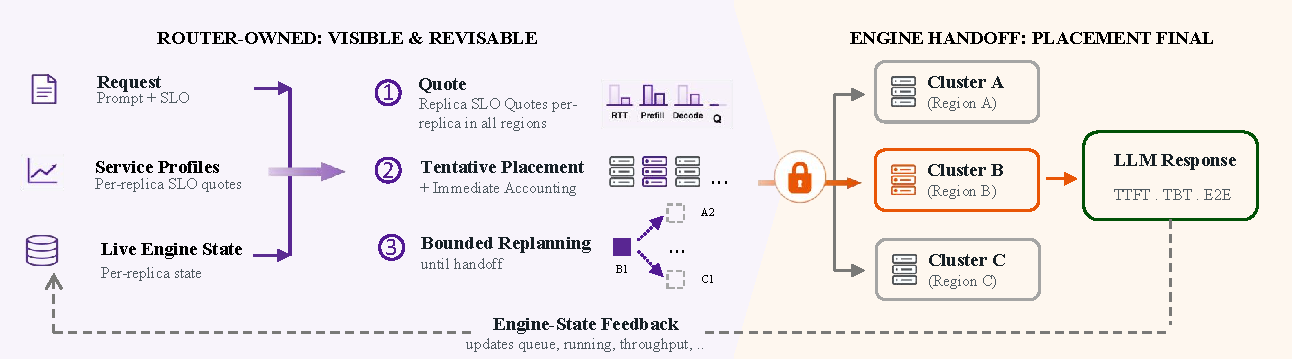
\includegraphics[width=\columnwidth]{figures/system.pdf}
    \caption{
    \textbf{RAVEL request lifecycle and ownership boundary.}
    On arrival, RAVEL constructs replica-specific SLO quotes, selects a
    tentative placement, and immediately accounts the request's prospective
    demand.
    While Router-owned, the request remains eligible for bounded reassignment,
    with tentative ownership and prospective accounting transferred together.
    Capacity-gated dispatch initiates engine handoff; only successful handoff
    makes placement final.
    Live engine state feeds back into subsequent quotes and accounting.
    }
    \label{fig:ravel-overview}
\end{figure}


\subsection{Overview}
\label{sec:design:overview}

RAVEL realizes the separation exposed by
Figure~\ref{fig:motivation}: arrival establishes demand visibility, Router
ownership preserves placement revisability, and successful engine handoff
establishes finality.
While Router-owned, each request has exactly one tentative replica owner and
one prospective demand representation.
Its destination may change as new demand or serving-state feedback arrives,
but its demand remains visible throughout.
After successful handoff, the serving engine owns the request and its
geographic placement is no longer revised.

Figure~\ref{fig:ravel-overview} summarizes this lifecycle.
On arrival, RAVEL constructs request-specific SLO quotes for candidate
replicas, chooses an initial virtual placement, and immediately accounts the
request's prospective demand at that replica.
Subsequent arrivals and engine feedback may trigger bounded replanning over a
cohort of still-Router-owned requests.
A reassignment moves both tentative ownership and replica-dependent
prospective demand to the new replica.
Requests approach execution through a shallow capacity-gated dispatch
frontier; a rejected handoff restores Router ownership, whereas a successful
handoff transfers ownership to the serving engine and makes placement final.

The design maintains three classes of invariants.
\emph{Single representation:} each Router-owned request has exactly one
tentative owner and one prospective demand representation.
\emph{Bounded mobility:} only Router-owned requests may move, and replanning is
causal and bounded in both time and scope.
\emph{Explicit finality:} tentative placement, hold expiration, and dispatch
eligibility do not commit a request; only successful engine handoff does.
The following sections describe how RAVEL enforces these properties.


\subsection{Replica SLO Quotes}
\label{sec:design:feasibility}

Revisability is useful only if the Router can determine which replicas remain
SLO-feasible for each request.
Because regional capacity is request-dependent
(Section~\ref{sec:problem:feasibility}), RAVEL represents each candidate using
a request- and replica-specific SLO quote rather than a request-independent
load score.
A quote summarizes whether the request is predicted to satisfy its applicable
SLOs, the request-specific objective used to rank viable targets, and
secondary capacity-pressure information.

Let $c\in\mathcal{C}$ denote a serving cluster,
$\mathcal{R}_c$ its replicas, $c(r)$ the cluster containing replica $r$, and
$\mathcal{R}=\bigcup_c\mathcal{R}_c$.
For request $i$ and candidate replica $r$, RAVEL constructs
\begin{equation}
    Q_{i,r}(t)
    =
    \left(
        \Phi_{i,r}(t),
        \widehat{T}^{\mathrm{obj}}_{i,r}(t),
        \mathbf{z}_{i,r}(t)
    \right),
    \label{eq:ravel-quote}
\end{equation}
where $\Phi_{i,r}(t)$ indicates whether all applicable SLO constraints are
predicted to hold,
$\widehat{T}^{\mathrm{obj}}_{i,r}(t)$ is the request-class-specific objective
used for ordering and slack calculations, and
$\mathbf{z}_{i,r}(t)$ contains secondary capacity-pressure signals.
Quotes use only information causally available at time $t$ and are online
predictions rather than formal SLO guarantees.

RAVEL combines calibrated cluster-level service profiles with live and
prospective replica state.
At active Decode concurrency $n$, it models Prefill service for prompt size
$p$ as
$P_{c,n}(p)=b_{c,n}+a_{c,n}p$ and uses $d_c(n)$ for calibrated
post-first-token Decode time per token.
For request $i$ and replica $r$, let
$\widehat{S}^{\mathrm{pre}}_{i,r}$ denote predicted Prefill-side service delay,
including live engine Prefill debt, Router-owned prompt work ahead of $i$, the
request's own prompt demand, and tentative assignments made earlier in the
same planning pass.
RAVEL predicts
\begin{equation}
    \widehat{\mathrm{TTFT}}_{i,r}(t)
    =
    (t-a_i)
    +
    \rho_{o_i,c(r)}
    +
    \widehat{S}^{\mathrm{pre}}_{i,r},
    \label{eq:ravel-ttft}
\end{equation}
where $a_i$ is request arrival time and
$\rho_{o_i,c(r)}$ is directed WAN delay from origin $o_i$ to cluster $c(r)$.
The elapsed term directly charges time already spent under Router ownership,
so a previously feasible replica may become infeasible as request slack
shrinks.

RAVEL evaluates each SLO according to its semantics rather than collapsing
them into one latency score.
For LATENCY requests, TTFT and TBT feasibility are checked independently:
a lower predicted TTFT cannot compensate for a predicted TBT violation.
For completion-oriented requests, RAVEL separates a conservative
output-demand estimate used for feasibility from an expected estimate used
for shared service-pressure accounting, avoiding both optimistic admission
and systematic over-accounting.
Appendix~\ref{sec:appendix:quotes} gives the complete TTFT, TBT, and completion
equations, calibration procedure, runtime sources, and fallback rules.


\subsection{Immediate and Transferable Demand Accounting}
\label{sec:design:accounting}

Figure~\ref{fig:motivation} shows that placement revisability loses much of its
value when already-arrived work is withheld from capacity accounting.
RAVEL therefore makes tentative demand visible immediately and exactly once,
without making its placement final.
Every Router-owned request is associated with one tentative replica queue and
one set of replica-dependent prospective charges.

When request $i$ receives a virtual placement at replica $r$, it immediately
enters $r$'s Router-owned queue.
Its prompt contributes to the queue-ahead Prefill work observed by later
quotes, including quotes constructed later in the same planning pass.
The Router also maintains lightweight prospective completion-service and
LATENCY/TBT pressure signals.
These signals complement, rather than replace, the replica's live pending and
running engine state.

Replanning must preserve this visibility as placement changes.
If $i$ moves from replica $r$ to $r'$, RAVEL atomically transfers its tentative
queue ownership and recomputes the replica-dependent prospective charges for
$r'$.
The serialized control path ensures that a planning snapshot observes
request $i$ at exactly one tentative owner---never at both replicas and never
at neither.
The destination then exposes the transferred demand to all subsequent quote
and placement decisions.

Visibility also remains continuous across the ownership boundary.
Successful handoff ends Router queue ownership, after which committed work is
represented by live engine state and an active-service charge until terminal
completion.
A rejected handoff restores the Router-owned prospective state.
These transitions establish RAVEL's central accounting invariant:
\emph{tentative work is immediately visible, but visibility does not make its
placement final}.
Appendix~\ref{sec:appendix:accounting} gives exact charge definitions, transfer
operations, deduplication rules, lifecycle transitions, and stale-callback
protection.


\subsection{Bounded Pre-Handoff Replanning}
\label{sec:design:replanning}

Later arrivals can expose stale allocations, but exploiting them requires
revisability to remain bounded in both time and scope.
RAVEL therefore reconsiders only Router-owned requests whose placements can
still change.
Committed work remains fixed but continues to affect later quotes through live
engine state.
Planning is event-driven, serialized, and coalesced so that each pass operates
on a consistent prospective view.

\paragraph{Bounding the revisable interval.}
For selected non-LATENCY requests, RAVEL preserves a short observation window
before dispatch.
Importantly, the request is already tentatively placed and prospectively
accounted during this interval; the hold changes only how long the placement
remains revisable.

Let
\[
\sigma_i^{\mathrm{arr}}
=
\max\!\left\{
0,\,
\Delta_i-
\min_r\widehat{T}^{\mathrm{obj}}_{i,r}(a_i)
\right\}
\]
denote the request's arrival-time planning slack, where $\Delta_i$ is its
applicable TTFT or completion planning budget.
RAVEL sets
\begin{equation}
    h_i
    =
    \begin{cases}
        \min\!\left\{
            \rho_i^{\min},
            \sigma_i^{\mathrm{arr}}
        \right\},
        & \text{if $i$ is hold-eligible},\\
        0,
        & \text{otherwise},
    \end{cases}
    \label{eq:ravel-mobility-hold}
\end{equation}
where $\rho_i^{\min}$ is the minimum positive RTT to a remote serving cluster.
Thus, deliberate observation is bounded by both a network timescale and the
request's available planning slack.
LATENCY requests use $h_i=0$.
Expiration of $h_i$ makes the request dispatch-eligible; it neither removes
its prospective accounting nor commits its placement.

\paragraph{Bounding replanning scope.}
Each planning pass considers a deterministic deadline-first prefix of at most
$K$ movable requests.
Requests outside the cohort retain their tentative owners and enter the
planning snapshot as fixed context.
Within the cohort, each selected placement immediately updates pass-local
prospective state before the next request is evaluated.
With $R=|\mathcal{R}|$ candidate replicas and effective cohort bound
$K_{\mathrm{eff}}$, one greedy pass performs
$O(K_{\mathrm{eff}}R)$ request--replica quote comparisons.
Under sustained completion pressure, RAVEL may expand the effective cohort
within the deployment's finite sequence capacity; this changes how much
Router-owned work is reconsidered, not the placement or commitment semantics.

\paragraph{Choosing initial and revised placements.}
RAVEL uses the same SLO-aware placement rule for an arrival and for requests
reconsidered during replanning.
If at least one replica is predicted feasible, the Router selects among
feasible targets.
If none is feasible, it first minimizes normalized predicted SLO violation.
Remaining choices are ordered lexicographically by
\emph{SLO safety}, \emph{capacity pressure}, and finally
\emph{efficiency and stability}.
The capacity-pressure tier discourages broadly substitutable requests from
occupying scarce SLO-feasible capacity, while lower-priority signals include
predicted service cost, movement, prefix locality, and deterministic
tie-breaking.
Consequently, locality or stability cannot override an avoidable predicted
SLO miss.

Replanning applies this same rule to the bounded movable cohort.
After each target is selected, RAVEL immediately updates pass-local
prospective state so that later requests in the same pass observe the demand
created by earlier tentative choices.
Algorithm~\ref{alg:ravel-control} summarizes the resulting Router control loop.
Appendix~\ref{sec:appendix:replanning} and
Appendix~\ref{sec:appendix:placement-key} provide the exact trigger predicates,
eligibility rules, cohort ordering, reassignment limits, and placement key.


\begin{algorithm}[t]
\caption{\textsc{RAVEL} Router Control Loop}
\label{alg:ravel-control}
\small

\Fn{\textnormal{\textsc{OnArrival}}($i$)}{
    $Q_i \gets \textsc{QuoteReplicas}(i)$\;
    $r_i \gets \textsc{SLOAwarePlace}(i,Q_i)$\;
    \textsc{AssignAndAccount}($i,r_i$)\;
    \tcp{Visible immediately; placement remains tentative}

    $h_i \gets \textsc{MobilityHold}(i,Q_i)$\;
    \If{$h_i = 0$}{
        \textsc{RequestReplan}()\;
    }
    \Else{
        \textsc{ArmReplan}($h_i$)\;
    }
}

\BlankLine

\Fn{\textnormal{\textsc{Replan}}()}{
    $C \gets \textsc{BoundedMovableCohort}()$\;
    \tcp{Only Router-owned requests are movable}

    \For{$i \in C$}{
        $Q_i \gets \textsc{QuoteReplicas}(i)$\;
        $r_i' \gets \textsc{SLOAwarePlace}(i,Q_i)$\;
        \textsc{TransferOrRefresh}($i,r_i'$)\;
        \tcp{Update prospective state before the next request}
    }
}

\BlankLine

\Fn{\textnormal{\textsc{Dispatch}}($i$)}{
    \If{\textsc{Held}($i$) \textbf{or} \textsc{FrontierBlocks}($i$)}{
        \Return\;
    }

    $r_i \gets \textsc{TentativeOwner}(i)$\;
    $s \gets \textsc{AttemptHandoff}(i,r_i)$\;

    \If{$s=\textsc{Rejected}$}{
        \textsc{RestoreRouterOwnership}($i,r_i$)\;
    }
    \ElseIf{$s=\textsc{Committed}$}{
        \textsc{FinalizePlacement}($i,r_i$)\;
        \tcp{Successful handoff is the commitment boundary}
    }
}
\end{algorithm}


\subsection{Commitment and Execution Protection}
\label{sec:design:commitment}

Revisability must end at a precise boundary, and execution after that boundary
must preserve the assumptions under which the placement was judged feasible.
RAVEL therefore separates approaching commitment, committing ownership, and
protecting execution after handoff.

\paragraph{Capacity-gated dispatch.}
A shallow dispatch frontier limits how much Router-owned work approaches
commitment at once.
The frontier determines \emph{when} a tentatively placed request may be handed
to its engine; it does not choose \emph{where} the request executes.
Work behind the frontier remains tentatively placed, prospectively accounted,
and eligible for replanning.
A request becomes dispatch-eligible when its tentative replica has sufficient
engine headroom, bounding proximity to commitment without introducing a
separate placement or admission policy.
Appendix~\ref{sec:appendix:frontier} gives the frontier construction and
headroom test.

\paragraph{Engine handoff as the commitment boundary.}
Commitment is an ownership transition rather than a timer or queue event.
For a dispatch-eligible request, RAVEL attempts replica registration followed
by creation of the engine-facing posting task.
Only successful completion of the handoff transfers the request from
Router-owned, revisable state to engine-owned, final state.
Failures before this boundary restore or clean the Router-owned state; failures
after handoff terminate the committed attempt without reopening geographic
placement.
Attempt identifiers prevent stale callbacks from modifying newer ownership or
accounting state.
Thus, tentative placement, hold expiration, dispatch eligibility, and temporary
removal from a Router queue are all non-commitment events.

\paragraph{Preserving quote assumptions at the engine.}
Final placement remains useful only if local execution preserves the service
conditions under which that placement was considered feasible.
In particular, Prefill--Decode interference can invalidate a TBT-feasible
quote after handoff.
When Chunked Prefill is enabled and LATENCY Decode is active, RAVEL exports the
tightest applicable TBT requirement and deadline metadata to a local serving
adapter.
The adapter combines this requirement with a calibrated conservative Prefill
envelope to bound the next Prefill quantum and gives LATENCY requests
deadline/TBT-aware local priority, while non-LATENCY work retains stable FCFS
behavior.
This mechanism protects the execution assumptions underlying replica quotes;
it does not introduce another geographic placement decision.

Together, these mechanisms complete the lifecycle derived in
Section~\ref{sec:problem}:
\emph{arrival makes demand visible, Router ownership keeps placement revisable,
and successful engine handoff makes placement final}.
Appendix~\ref{sec:appendix:handoff} and
Appendix~\ref{sec:appendix:tbt-control} give the complete ownership state
machine, failure transitions, activation rules, and local scheduling details.

\section{Implementation}
\label{sec:implementation}

We implement RAVEL in Python as an asynchronous control layer in front of
geo-distributed vLLM serving replicas~\cite{vllm}.
Our implementation targets vLLM~0.8.5.post1 and its frozen V0 scheduler
contract.
All control-plane operations that modify Router-owned queues, perform
replanning, or initiate dispatch are serialized by a single
\texttt{asyncio} scheduler lock.
New arrivals, mobility-hold expirations, engine feedback, and explicit
replanning requests therefore enter the same serialized scheduling path,
preventing concurrent passes from racing on tentative ownership or
prospective accounting.
Terminal callbacks may asynchronously release tracked service charges, but
any resulting replanning again enters this serialized path.

\paragraph{Serving profiles.}
RAVEL derives serving estimates from externally calibrated schema-v2 profiles
rather than hard-coded token rates.
Each profile carries an engine fingerprint and is bound to one serving cluster;
formal runs require a valid external profile for every cluster.
At runtime, RAVEL linearly interpolates Prefill and Decode measurements between
calibrated concurrency points and clamps queries outside the measured range to
the nearest endpoint.
The engine adapter additionally constructs a conservative Prefill envelope
from the maximum calibrated slope and intercept across concurrency levels.
For multi-stage completion requests, the Router may also load an offline
semantic output profile indexed only by request-visible workflow metadata,
such as $(\textit{stage\_id},\textit{stage\_num})$.
Neither profile exposes future arrivals or realized output length.

\paragraph{vLLM integration and local TBT control.}
RAVEL integrates with vLLM without modifying its source tree.
At process startup, a lightweight adapter feature-detects and wraps
\texttt{Scheduler.\_get\_priority} and
\texttt{Scheduler.\_schedule\_chunked\_prefill}.
If either required hook is unavailable, startup fails rather than silently
disabling RAVEL's local controls.
For LATENCY requests, the adapter encodes a Router-derived deadline-order key
together with the applicable TBT requirement in a reserved priority range;
non-LATENCY requests in the mixed path retain ordinary FCFS priority.
When LATENCY Decode is active, the adapter combines the tightest active TBT
requirement with the conservative Prefill envelope to derive a block-aligned
bound on the next Prefill quantum.
It temporarily reduces \texttt{max\_num\_batched\_tokens} for that
Chunked-Prefill scheduling iteration and restores the configured value in a
\texttt{finally} block.
The bound therefore affects only the current local scheduling decision and
does not introduce a separate Router-level placement policy.

\paragraph{Asynchronous handoff and failure handling.}
Engine handoff is implemented as an explicit asynchronous ownership
transition.
After Router-side admission and budget checks succeed, the target replica
first registers the request, after which RAVEL creates and tracks the
corresponding engine-facing posting task.
Successful replica registration together with successful posting-task
creation constitutes the handoff defined in
Section~\ref{sec:design:commitment}; only then does placement become final.

If replica registration is rejected, the request is restored to its
Router-owned queue together with its prospective state and remains eligible
for the ordinary mobility and replanning rules.
Failures while creating or executing an engine-facing posting task are
surfaced to the control plane rather than silently converted into new
Router-level placements.
Posting attempts carry attempt identifiers so that delayed callbacks from an
older attempt cannot modify ownership or accounting associated with a newer
one.

After successful handoff, replica-reported pending and running state continues
to inform subsequent Router quotes.
The corresponding active-service charge remains visible until terminal
completion.
At request termination, RAVEL releases that charge and requests another
serialized scheduling pass so that newly available capacity can affect
requests that remain Router-owned.


\begin{figure*}[t]
    \centering
    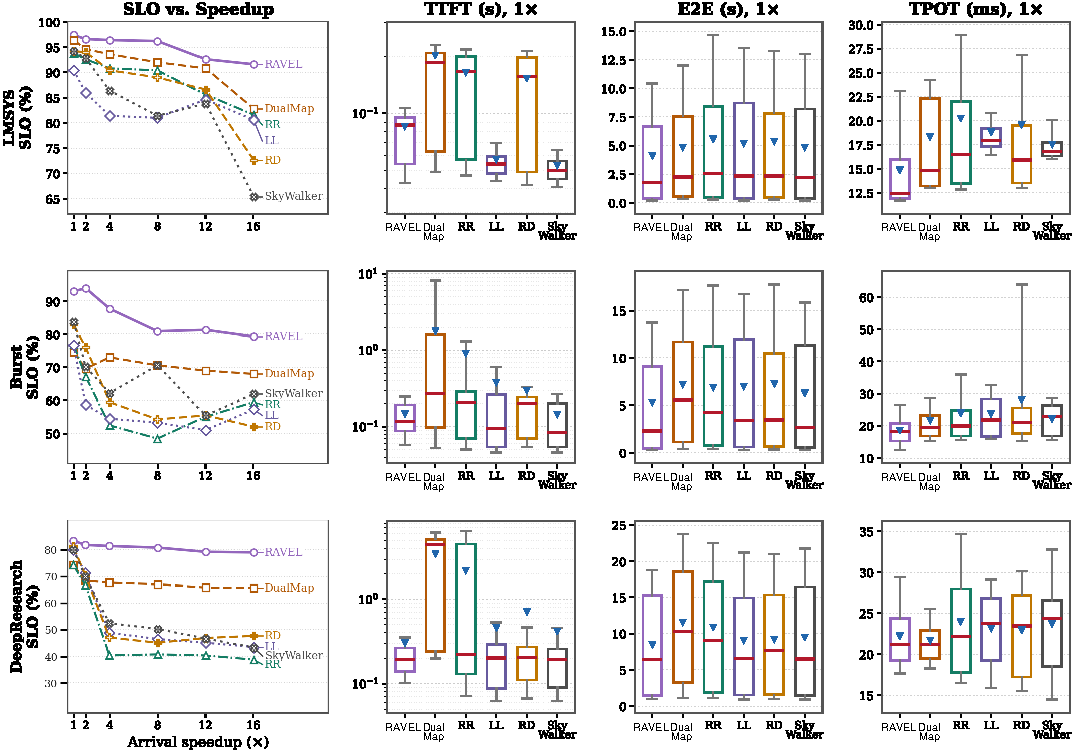
\includegraphics[width=\textwidth]{figures/end_to_end.pdf}
    \caption{
RAVEL preserves higher request-level SLO attainment as offered load increases.
Rows correspond to LMSYS, Burst, and DeepResearch.
The first column varies arrival speedup from $1\times$ to $16\times$; the
remaining columns report TTFT, end-to-end latency, and TPOT distributions at
$1\times$ load.
RAVEL consistently achieves the highest SLO attainment across the evaluated
workloads and loads, without requiring uniformly lower values of every
individual latency metric.
}
    \label{fig:main-results}
\end{figure*}

\section{Evaluation}
\subsection{Experimental Setup}
\label{sec:eval:setup}

\paragraph{Testbed and replay.}
We deploy five Qwen3-1.7B serving replicas across three clusters in a
2/2/1 configuration.  Each replica runs on an NVIDIA GeForce RTX~4090 GPU
with bfloat16 precision using vLLM~0.8.5.post1 (V0).
The final experiments use physical WAN transport rather than synthetic
latency injection; measured directed inter-cluster RTTs range from
10.1 to 37.9\,ms.
Table~\ref{tab:eval-setup} summarizes the common serving configuration.
All policies use the same hardware, topology, and base vLLM configuration;
RAVEL's TBT-aware local control is part of the system evaluated in
Section~\ref{sec:eval:mechanism}.

We replay requests \emph{open-loop}.  For an arrival-rate speedup $s$, we
scale trace inter-arrival times by $1/s$, so control-plane overhead cannot
backpressure the offered load.
We evaluate $1\times$, $2\times$, $4\times$, $8\times$, $12\times$, and
$16\times$ arrival rates, with 500 requests in every
policy--workload--load cell.
Before formal measurement, we warm all backends using the same execution
path.  Before each cell, we reset the prefix cache on every replica,
preventing cached state from carrying across policy comparisons.

\begin{table}[t]
\centering
\small
\caption{Evaluation testbed and serving configuration.}
\label{tab:eval-setup}
\begin{tabular}{@{}ll@{}}
\toprule
\textbf{Dimension} & \textbf{Configuration} \\
\midrule
Model               & Qwen3-1.7B \\
GPU                 & NVIDIA GeForce RTX 4090 \\
Precision           & bfloat16 \\
Serving engine      & vLLM 0.8.5.post1 (V0) \\
Deployment          & 5 replicas / 3 clusters (2/2/1) \\
Network             & Physical WAN \\
Inter-cluster RTT   & 10.1--37.9\,ms (directed) \\
Max. sequences      & 64 per replica \\
Max. batched tokens & 16,384 \\
Prefix caching      & Enabled \\
Chunked Prefill     & Enabled \\
Requests per cell   & 500 \\
Arrival speedup     & $1,2,4,8,12,16\times$ \\
\bottomrule
\end{tabular}
\end{table}

\paragraph{Workloads.}
We evaluate three workload regimes that expose different forms of contention
in geo-distributed serving.
\emph{LMSYS} contains heterogeneous conversational requests with diverse
prompt and response sizes.
\emph{Burst} uses the same 500 request contents as LMSYS but replaces their
arrival timestamps with BurstGPT timestamps.
This controlled construction isolates short-horizon arrival contention from
changes in the request-content distribution.
\emph{DeepResearch} is derived from multi-stage, completion-oriented
workflows.  We flatten branch requests by arrival time and evaluate the first
500 branch requests using request-level completion SLOs; the selected trace
does not define a workflow-level task SLO.
For DeepResearch, RAVEL's semantic output profile is constructed exclusively
from the designated training split and never uses the realized output of an
evaluation request.
Together, the workloads cover heterogeneous conversational traffic,
transient burst contention, and sustained completion-oriented demand.

\paragraph{SLOs.}
We use the JITServe-style heterogeneous-SLO construction implemented by our
evaluation runner.
The base budgets are 0.8\,s for TTFT, 80\,ms for TBT, and 8\,s for
end-to-end completion, with a request-specific multiplier from
$1\times$ to $4\times$.
For LMSYS and Burst, the released class-assignment procedure produces
181 LATENCY, 301 THROUGHPUT, and 18 COLLECTIVE requests in each
500-request trace (seed 42); DeepResearch branch requests are COLLECTIVE.
A LATENCY request succeeds only if its TTFT and every measured TBT satisfy
their respective budgets.
THROUGHPUT and COLLECTIVE requests instead succeed when their end-to-end
latency satisfies the corresponding completion budget.

\paragraph{Baselines.}
We compare RAVEL against five routing policies.
\emph{Round Robin (RR)} is stateless and distributes incoming requests
across serving replicas in round-robin order.
\emph{Least Load (LL)} tracks the number of outstanding requests at each
replica and routes each new request to the replica with the smallest
outstanding-request count.
\emph{Random (RD)} independently selects a serving replica at random for
each incoming request.
\emph{DualMap} jointly considers cache affinity and serving load and
rebalances traffic when affinity-driven placements become hotspots.
\emph{SkyWalker} performs locality-aware cross-region load balancing,
preferring available local capacity and redirecting requests when local
replicas become saturated while preserving prefix locality.
All policies replay identical request records over the same serving topology
and base engine configuration; each baseline uses only the state prescribed
by its routing policy.

\paragraph{Metrics.}
Our primary metric is \emph{request-level SLO attainment}, i.e., the
fraction of requests satisfying the class-specific success criteria above.
We additionally report time to first token (TTFT), time per output token
(TPOT), and end-to-end request latency to separate application-level SLO
outcomes from individual latency components.
For LATENCY requests, we additionally report TBT violations when analyzing
streaming performance.
All evaluated cells complete all 500 requests, and SLO misses remain in the
denominator.




\subsection{End-to-End Performance}
\label{sec:eval:e2e}

Figure~\ref{fig:main-results} summarizes RAVEL's end-to-end performance
across the three workload regimes.
The first column reports request-level SLO attainment as the offered load
increases from $1\times$ to $16\times$.
The remaining columns show the distributions of TTFT, end-to-end latency,
and TPOT at nominal load.
Together, these results characterize RAVEL's SLO attainment under increasing
contention and its latency behavior at nominal load.

\textbf{RAVEL sustains higher SLO attainment under load.}
RAVEL achieves the highest request-level SLO attainment across all three
workloads and every evaluated arrival rate.
The separation is particularly pronounced in several high-contention
settings.
At $16\times$ load, RAVEL attains 91.6\% of request SLOs on LMSYS,
compared with 82.8\% for the best-SLO baseline, DualMap;
79.2\% on Burst, compared with 62.0\% for SkyWalker; and
64.2\% on DeepResearch, compared with 47.6\% for RD.
These correspond to gains of 8.8, 17.2, and 16.6 percentage points,
respectively.
RAVEL therefore retains substantial advantages even when offered load
creates severe contention for serving capacity.

The contrast between LMSYS and Burst provides a controlled view of this
contention.
Burst preserves the same request contents as LMSYS and changes only their
arrival timestamps.
RAVEL's larger advantage on Burst therefore coincides with greater
short-horizon arrival contention rather than a change in the prompt or
response distribution.
The DeepResearch results further show that RAVEL's gains extend beyond mixed
interactive traffic to sustained completion-oriented demand.

\textbf{RAVEL improves SLO attainment while maintaining competitive
latency.}
At nominal load, RAVEL's TTFT, end-to-end latency, and TPOT distributions
remain competitive with the baselines across all three workloads.
Its SLO gains under stress are also accompanied by favorable P95 latency.
At $16\times$ load, RAVEL achieves both higher request-level SLO attainment
and lower P95 TTFT and P95 end-to-end latency than the best-SLO baseline for
each workload.
For example, on Burst, RAVEL reduces P95 TTFT from 8.70\,s to 2.68\,s and
P95 end-to-end latency from 28.68\,s to 18.78\,s relative to SkyWalker,
while increasing SLO attainment from 62.0\% to 79.2\%.
These results highlight the distinction between optimizing a single latency
statistic and maximizing class-specific request-level SLO attainment.

These end-to-end results establish RAVEL's performance benefit but do not
attribute it to individual mechanisms.
Section~\ref{sec:eval:mechanism} next isolates pre-handoff revisability and
RAVEL's SLO-specific execution controls.

\begin{figure*}[t]
    \centering
    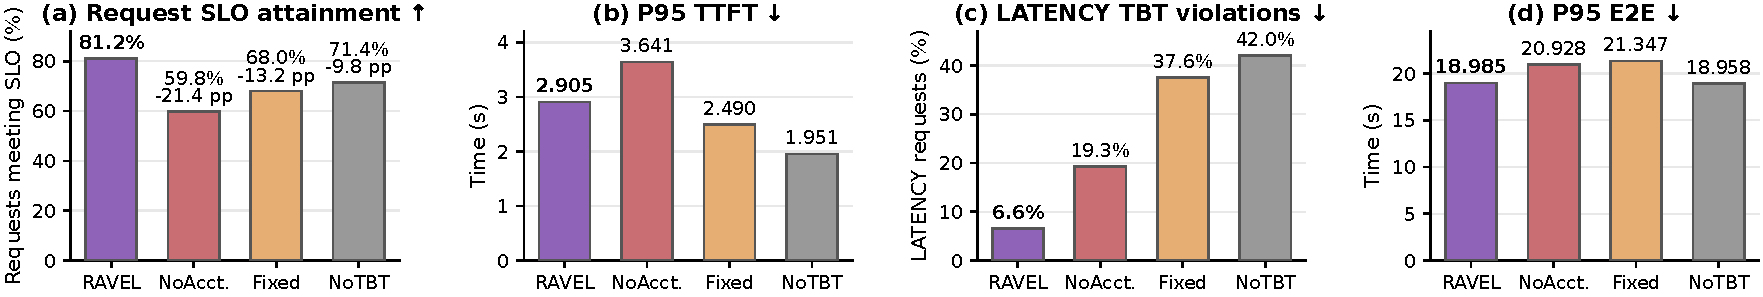
\includegraphics[width=\textwidth]{figures/mechanism_breakdown.pdf}
    \caption{
\textbf{Mechanism breakdown on Burst at $12\times$ load.}
\emph{FixedPlacement} retains immediate demand accounting but disables
pre-handoff reassignment; \emph{NoTBTGuard} retains Router-side RAVEL
placement but disables the local TBT-aware Chunked-Prefill guard.
We report (a) request-level SLO attainment, (b) P95 TTFT,
(c) the fraction of LATENCY requests with at least one TBT violation, and
(d) P95 end-to-end latency.
Both pre-handoff revisability and local TBT protection materially contribute
to RAVEL's SLO gains.
}
    \label{fig:mechanism-breakdown}
\end{figure*}
\subsection{Mechanism Breakdown}
\label{sec:eval:mechanism}

We next isolate the mechanisms behind RAVEL's end-to-end gains using the
Burst workload at $12\times$ load, where short-horizon contention is strong
while the request contents remain identical to LMSYS.
Figure~\ref{fig:mechanism-breakdown} compares full RAVEL with two ablations:
\emph{FixedPlacement}, which preserves immediate prospective demand
accounting but prevents a tentative replica assignment from changing before
engine handoff, and \emph{NoTBTGuard}, which preserves the global RAVEL
routing policy but disables the local TBT-aware Chunked-Prefill guard.
Each variant processes the same 500-request trace.
The TBT-violation metric is computed over the 181 LATENCY requests in that
trace.

\textbf{Pre-handoff revisability materially improves SLO attainment.}
Freezing the initial tentative placement reduces request-level SLO attainment
from 81.2\% to 68.0\%, a 13.2 percentage-point drop
(Figure~\ref{fig:mechanism-breakdown}a).
Importantly, FixedPlacement still accounts arrived demand immediately, so
later requests observe the load created by earlier tentative assignments.
What it removes is the ability to act on newly revealed demand by revising
those earlier assignments.
The resulting degradation therefore shows that demand visibility alone is
insufficient: earlier placements must remain revisable while they are still
under Router control.
This effect is also visible in streaming performance, where the LATENCY TBT
violation rate increases from 6.6\% under RAVEL to 37.6\% under
FixedPlacement (Figure~\ref{fig:mechanism-breakdown}c).

The result is particularly notable because FixedPlacement does not have worse
TTFT.
Its P95 TTFT is 2.49\,s, compared with 2.91\,s for RAVEL
(Figure~\ref{fig:mechanism-breakdown}b), yet it satisfies substantially fewer
complete request SLOs.
This reinforces the distinction between optimizing one latency component and
preserving the joint SLO constraints that determine whether a request
actually succeeds.

\textbf{Global placement and local TBT protection address complementary
sources of SLO loss.}
Disabling RAVEL's local TBT guard lowers request-level SLO attainment from
81.2\% to 71.4\%, a 9.8 percentage-point reduction.
The clearest change is in the LATENCY requests: their TBT violation rate rises
from 6.6\% to 42.0\%.
At the same time, NoTBTGuard has a lower P95 TTFT than RAVEL
(1.95\,s versus 2.91\,s) and nearly identical P95 end-to-end latency
(18.96\,s versus 18.99\,s).
The degradation is therefore concentrated in the streaming constraint that
the guard is designed to protect rather than in a broad increase in
completion latency.
These results show that selecting an appropriate replica globally is not
sufficient by itself; the local serving path must also bound Prefill
interference in accordance with activ e TBT requirements.

Together with the LateBind experiment in Figure~\ref{fig:motivation}, these
ablations separate the two parts of RAVEL's core design.
Late binding delays commitment but also delays regional demand attribution,
whereas FixedPlacement makes demand visible immediately but removes
pre-handoff revisability.
RAVEL combines both properties: arrived demand influences subsequent
placement decisions immediately, while tentative assignments remain
changeable until engine handoff.


\begin{figure}[t]
    \centering
    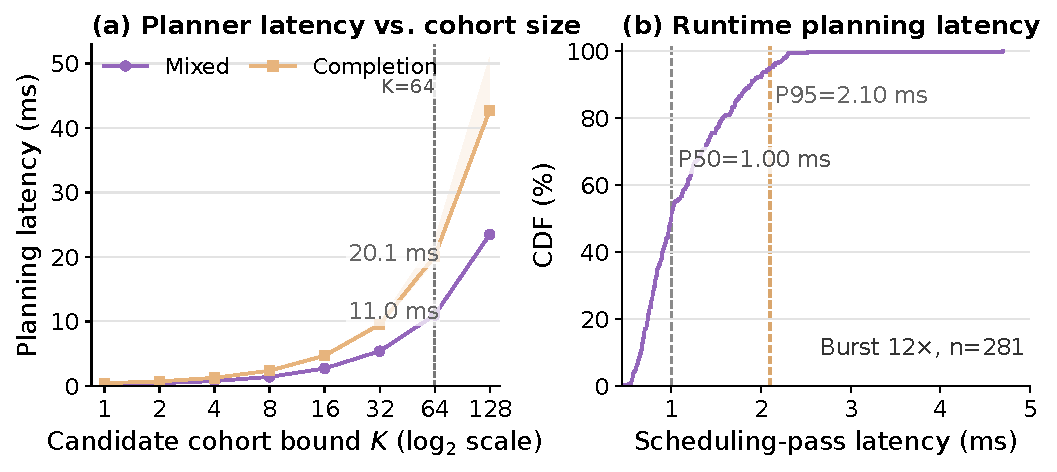
\includegraphics[width=\columnwidth]{figures/planner_overhead.pdf}
    \caption{
    \textbf{RAVEL control-plane scalability and runtime overhead.}
    (a) Planner latency versus candidate-cohort size for the mixed-traffic
    WorkYield and completion OnTimeSet planners; the dashed line marks the
    mixed-path bound $K=64$.
    (b) CDF of scheduling-pass latency in a 500-request Burst run at
    $12\times$ load.
    The runtime median/P95 are 1.00/2.10\,ms, while the mean/P95 candidate
    cohort sizes are 3.65/7 requests.
    }
    \label{fig:planner-overhead}
\end{figure}

\subsection{Control-Plane Scalability and Overhead}
\label{sec:eval:overhead}

We finally evaluate whether RAVEL's pre-handoff replanning can operate on the
online serving timescale.
Figure~\ref{fig:planner-overhead} separates two questions.
First, we measure how planner latency scales with the size of the candidate
cohort using states derived from the Burst and DeepResearch traces.
For each planner and cohort size, we run five warm-up iterations followed by
50 measured repetitions on an isolated CPU.
Second, we instrument an end-to-end Burst run at $12\times$ load and report
the distribution of planning latency observed during actual execution.

\textbf{Bounded replanning keeps multi-request planning tractable.}
Figure~\ref{fig:planner-overhead}a varies the candidate cohort from 1 to
128 requests for both RAVEL planning paths.
Planning cost increases with cohort size, with the completion planner
consistently more expensive because it additionally considers protected-set
replacement and deferred-request retries.
At RAVEL's normal cohort bound of $K=64$, the median planning latency is
10.99\,ms for the mixed planner and 20.10\,ms for the completion planner;
their P95 latencies are 11.18\,ms and 22.61\,ms, respectively.
Even when the replayed cohort is increased to 128 requests, median latency
remains 23.47\,ms for mixed traffic and 42.75\,ms for completion traffic.
These measurements show the role of the cohort bound: RAVEL does not require
multi-request optimization over the entire Router-owned queue, but confines
the more expensive placement computation to an explicitly bounded working
set.

\textbf{Online planning usually operates far below the configured bound.}
Figure~\ref{fig:planner-overhead}b reports all 281 planning passes from a
500-request Burst run at $12\times$ load.
The median planning latency is 1.00\,ms, with P95 and P99 latencies of
2.10\,ms and 2.30\,ms, respectively; the maximum observed pass takes
4.70\,ms.
The reason actual costs are substantially below the $K=64$ replay point is
that online cohorts are typically small: the mean cohort size is 3.65,
the P95 is 7, and the maximum observed cohort is 9.
Thus, the configured bound protects the control plane against unusually
large reversible sets, while the common online path replans only a small
number of requests at a time.

Overall, these results show that preserving pre-handoff placement
revisability does not require continuously solving a large global assignment
problem.
RAVEL instead performs bounded multi-request replanning when additional
information becomes available, and the measured online planning path remains
at millisecond-scale latency under the evaluated burst workload.

\section{Related Work}
\label{sec:related}

\paragraph{Distributed and geo-distributed LLM routing.}
Distributed LLM serving systems increasingly incorporate runtime load and
cache locality into request routing.
Preble jointly considers reusable KV state and computation load when
scheduling prompts across distributed replicas~\cite{preble}, while DualMap
balances cache affinity against load and performs hotspot-aware
rebalancing~\cite{dualmap}.
Recent systems explicitly target geographically distributed serving.
SkyWalker handles cross-region traffic while preserving KV-cache locality and
load balance~\cite{skylb};
GORGO incorporates WAN latency, queueing state, and Prefill/cache cost into
cross-region routing decisions~\cite{gorgo};
and recent work such as Solyx combines serving telemetry with WAN
measurements for per-request cross-site placement~\cite{solyx}.
Although these systems may redirect or rebalance traffic after an initial
choice, RAVEL differs in the control abstraction it exposes:
it explicitly couples \emph{immediate prospective demand accounting} with
\emph{pre-handoff placement revisability}.
An arrived request is accounted at a tentative replica immediately, while
that replica may still change until the request is handed off to the serving
engine.

\paragraph{SLO-aware LLM serving and application scheduling.}
Prior systems also adapt LLM execution to request-level latency and SLO
requirements.
Sarathi-Serve uses Chunked Prefill to reduce Prefill--Decode interference and
control TTFT and inter-token latency~\cite{sarathi}, while DistServe
disaggregates Prefill and Decode and provisions the two phases according to
TTFT and TPOT requirements~\cite{distserve}.
JITServe targets heterogeneous latency-, deadline-, and compound-request
SLOs, scheduling serving capacity from imprecise request information and
refining those estimates as generation progresses~\cite{jitserve}.
AdaServe instead customizes speculative decoding to per-request SLO
requirements~\cite{adaserve}.
Other systems exploit structure across related LLM calls:
Parrot exposes application-level semantic dependencies to coordinate
multi-request execution~\cite{parrot}, and Agentix treats agentic programs as
first-class scheduling entities to optimize program-level end-to-end
latency~\cite{agentix}.
Libra further partitions requests into cooperating micro-requests and combines
global split-point decisions with local SLO-aware batching to balance dynamic
serving load across instances~\cite{libra}.
RAVEL applies the same broad principle of request-specific SLO awareness at a
different control layer: it uses WAN delay and replica serving state to
determine which geographic capacity remains viable for each request before
engine handoff.
Its local Prefill control complements this global decision by bounding
Prefill interference in accordance with latency-sensitive execution
constraints.

\paragraph{Dynamic reassignment and migration.}
Serving systems can also revise placement after an initial assignment.
Llumnix dynamically reschedules requests across model instances and uses live
migration to improve load balancing and isolation, mitigate resource
fragmentation, and differentiate request priorities and SLOs~\cite{llumnix}.
Such migration preserves placement flexibility even after execution state has
materialized.
RAVEL chooses an earlier control boundary: a request remains reassignable
while it is Router-owned, but its placement becomes final after successful
engine handoff.
Thus, RAVEL performs reassignment before changing placement would require
coordination with engine-managed request state, whereas migration systems
retain flexibility after that state already exists.
The two approaches are complementary: pre-handoff replanning can avoid some
state movement, while runtime migration can correct imbalance that emerges
after execution begins.

\section{Conclusion}

Geo-distributed LLM capacity is request-dependent: a region that is optional
for one request may be indispensable to another.
This makes irreversible arrival-time placement vulnerable to avoidable
allocation-induced SLO misses as later demand changes the opportunity cost of
regional capacity.

Our diagnosis shows that simply delaying commitment is insufficient.
At an 80-ms fixed late-binding delay, removing the direct waiting penalty
recovers only 0.6 percentage points of SLO attainment, whereas making held
requests immediately visible to prospective capacity accounting recovers
15.0 points.
The dominant recoverable loss therefore comes from delaying demand visibility
together with placement finality.

RAVEL separates these lifecycle decisions.
Requests enter capacity planning immediately through tentative placement and
prospective accounting, remain revisable while Router-owned, and become final
only after successful engine handoff.
Replica-specific SLO quotes, bounded pre-handoff replanning, and engine-local
protection make this separation practical.

On our physical-WAN vLLM deployment, RAVEL improves request-level SLO attainment
across conversational, bursty, and multi-stage workloads while retaining
millisecond-scale online planning overhead.
More broadly, preserving online flexibility need not require hiding
already-arrived work from the state used to make future decisions.

{\footnotesize
\bibliographystyle{acm}
\bibliography{sample}
}
\clearpage
\appendix
% --------------------------------------------------------------------------
% Draft-only helper.
% Delete \AppendixPlan and replace each scaffold with final prose before
% submission.
% --------------------------------------------------------------------------
\newcommand{\AppendixPlan}[3]{%
\paragraph{Question addressed.}
#1

\paragraph{Content to include.}
#2

\paragraph{Required evidence.}
#3
}


% ==========================================================================
% Appendix A
% ==========================================================================
\section{Detailed Design and Operational Semantics}
\label{app:design-details}


% --------------------------------------------------------------------------
\subsection{Common Request State and Notation}
\label{sec:appendix:state-model}

RAVEL separates \emph{placement ownership} from engine execution state.
Before successful engine handoff, a request is Router-owned: it has one
tentative replica, contributes prospective demand to that replica, and may be
replanned subject to the mobility rules below.
Successful engine handoff transfers ownership to the serving engine and makes
the geographic placement final.
Engine-side execution may subsequently move through Prefill, Decode,
completion, or failure states, but these events do not reopen geographic
placement.

For request $i$, $a_i$ denotes its Router arrival time, $o_i$ its client
region, and $r_i(t)$ its tentative replica while Router-owned.
The version counter $v_i$ protects versioned ownership and accounting
transfers, while $h_i^{\mathrm{att}}$ identifies the current engine attempt.
Attempt identifiers isolate asynchronous completion, cancellation, and cleanup
events across retries.

The Router-side transport path distinguishes
\texttt{WAITING\_MOVABLE} from the transient \texttt{COMMITTING} state around
engine handoff.
A dispatch claim enters \texttt{COMMITTING}; this is an ownership-transition
attempt rather than a second placement decision.
If target registration or pre-handoff posting setup fails, Router ownership is
restored or cleaned without reporting a committed placement.
Placement becomes final only after the target accepts registration and the
engine-facing posting task is created and tracked successfully.
RAVEL does not perform ordinary geographic rebinds after this boundary.

These operational rules refine the three invariant classes from
Section~\ref{sec:design:overview}.
Specifically, RAVEL ensures that
(i) each Router-owned request has exactly one tentative owner;
(ii) its prospective demand is represented exactly once and follows
reassignment;
(iii) only Router-owned requests may change geographic placement;
(iv) replanning is causal and bounded in observation time and cohort size;
and (v) only successful engine handoff commits placement.
Attempt identifiers additionally isolate asynchronous callbacks across
retries: a callback from attempt $h$ cannot modify state belonging to a newer
attempt $h'>h$.


% --------------------------------------------------------------------------
\subsection{Replica SLO Quote Construction}
\label{sec:appendix:quotes}

A placement decision consumes the causal quote
\begin{equation}
    Q_{i,r}(t)
    =
    \left(
        \Phi_{i,r}(t),
        \widehat{T}^{\mathrm{obj}}_{i,r}(t),
        \mathbf{z}_{i,r}(t)
    \right),
    \label{eq:appendix:quote-tuple}
\end{equation}
where $\Phi_{i,r}(t)$ is predicted SLO feasibility,
$\widehat{T}^{\mathrm{obj}}_{i,r}(t)$ is the class-specific ordering objective,
and $\mathbf{z}_{i,r}(t)$ contains secondary capacity-pressure and stability
signals.
Quotes use only information available at decision time and are not formal SLO
guarantees.
Their inputs include request-visible SLO metadata, directed WAN measurements,
calibrated per-cluster service profiles, observed engine state, Router-owned
queue state, and tentative assignments already selected in the current
planning pass.
The evaluated request's realized output length is never an input to its quote.

\paragraph{Calibrated service curves.}
For cluster $c$ and active Decode concurrency $n$, the service profile stores
an affine Prefill model
\begin{equation}
    P_{c,n}(p)=b_{c,n}+a_{c,n}p
    \label{eq:appendix:prefill-profile}
\end{equation}
and a measured post-first-token Decode time per token $d_c(n)$.
Profiles are calibrated independently for each serving cluster and carry an
engine fingerprint.
At runtime, RAVEL linearly interpolates between measured concurrency points
and clamps values outside the calibrated range to the nearest endpoint.
Because $P_{c,n}$ is measured while $n$ Decode sequences are active, RAVEL
does not add a separate ad-hoc Decode-interference penalty to the Prefill
estimate.

\paragraph{Queue-ahead Prefill expansion.}
Let $p_i$ be the full prompt-token charge of request $i$.
Without engine-certified cached-token residency, shadow prefix locality is used
only as a late placement tie-breaker and does not reduce $p_i$.

For candidate replica $r$, let $E_r$ denote observed engine-pending Prefill
tokens, $B_{i,r}$ the prompt tokens in Router-owned requests ordered no later
than $i$, $N_r^{\mathrm{eng}}$ the number of engine-pending requests, and
$N_{i,r}^{\mathrm{q}}$ the corresponding number of Router-owned queue-ahead
requests.
With $n_r$ currently running Decode sequences, RAVEL estimates
\begin{equation}
    \widehat{S}^{\mathrm{pre}}_{i,r}
    =
    a_{c(r),n_r}
    \left(E_r+B_{i,r}+p_i\right)
    +
    b_{c(r),n_r}
    \left(N_r^{\mathrm{eng}}+N_{i,r}^{\mathrm{q}}+1\right).
    \label{eq:appendix:prefill-service}
\end{equation}
During cohort replanning, $B_{i,r}$ and $N_{i,r}^{\mathrm{q}}$ additionally
include tentative assignments selected earlier in the same planning pass.
Thus, later candidates observe prospective work induced by earlier tentative
choices rather than a stale snapshot.

Using the notation of Section~\ref{sec:design:feasibility}, the TTFT estimate
is
\begin{equation}
    \widehat{\mathrm{TTFT}}_{i,r}(t)
    =
    (t-a_i)
    +
    \rho_{o_i,c(r)}
    +
    \widehat{S}^{\mathrm{pre}}_{i,r},
    \label{eq:appendix:ttft}
\end{equation}
where $\rho_{o_i,c(r)}$ is the directed client-to-cluster WAN delay.
The elapsed term explicitly charges Router observation time against the
request's remaining SLO budget.

\paragraph{Prospective Decode occupancy.}
Let $\mathcal{O}_r$ be the union of request identifiers visible in the
Router-owned queue, engine-pending set, and engine-running set at replica $r$.
RAVEL forms
\begin{equation}
    m_{i,r}
    =
    \max\!\left(
        1,\;
        \left|\mathcal{O}_r\cup\{i\}\right|,\;
        N_r^{\mathrm{q}}+N_r^{\mathrm{eng}}+N_r^{\mathrm{run}}
        +\mathbf{1}[i\notin\mathcal{O}_r]
    \right),
    \label{eq:appendix:prospective-seqs}
\end{equation}
and queries the calibrated Decode curve at $m_{i,r}$, clamping at the measured
profile endpoint.
The set term prevents the same request from being charged twice when lifecycle
views overlap.

\paragraph{LATENCY feasibility.}
For a LATENCY request with TTFT and TBT limits
$D_i^{\mathrm{TTFT}}$ and $D_i^{\mathrm{TBT}}$,
\begin{equation}
    \Phi^{\mathrm{lat}}_{i,r}(t)
    =
    \mathbf{1}\!\left[
        \widehat{\mathrm{TTFT}}_{i,r}(t)
        \le D_i^{\mathrm{TTFT}}
        \;\land\;
        d_{c(r)}(m_{i,r})
        \le D_i^{\mathrm{TBT}}
    \right].
    \label{eq:appendix:latency-feasible}
\end{equation}
The two constraints are evaluated independently: a low predicted TTFT cannot
compensate for a predicted TBT violation.

\paragraph{Completion feasibility and output demand.}
For completion-oriented requests, RAVEL distinguishes request-visible expected
output demand $L_i^{\mathrm{exp}}$ from conservative risk demand
$L_i^{\mathrm{risk}}$.
The corresponding completion estimates are
\begin{align}
    \widehat{T}^{\mathrm{exp}}_{i,r}(t)
    &=
    \widehat{\mathrm{TTFT}}_{i,r}(t)
    +
    \max(0,L_i^{\mathrm{exp}}-1)d_{c(r)}(m_{i,r}),
    \label{eq:appendix:completion-exp}\\
    \widehat{T}^{\mathrm{risk}}_{i,r}(t)
    &=
    \widehat{\mathrm{TTFT}}_{i,r}(t)
    +
    \max(0,L_i^{\mathrm{risk}}-1)d_{c(r)}(m_{i,r}).
    \label{eq:appendix:completion-risk}
\end{align}
Completion feasibility uses
\begin{equation}
    \Phi^{\mathrm{comp}}_{i,r}(t)
    =
    \mathbf{1}\!\left[
        \widehat{T}^{\mathrm{risk}}_{i,r}(t)
        \le D_i^{\mathrm{comp}}
    \right],
    \label{eq:appendix:completion-feasible}
\end{equation}
while $\widehat{T}^{\mathrm{exp}}_{i,r}$ represents expected shared service
pressure.

Ordinary feasibility always uses the conservative
$L_i^{\mathrm{risk}}$ estimate.
Under the completion-pressure path in
Section~\ref{sec:appendix:completion-pressure}, a held-out semantic profile may
replace the placement-time estimate of $L_i^{\mathrm{exp}}$ using only
request-visible workflow metadata.
It does not replace $L_i^{\mathrm{risk}}$, reveal future arrivals, or use the
evaluated request's realized output length.

\paragraph{Quote procedure.}
For completeness, a replica quote performs the following operations:
\begin{quote}
\textsc{QuoteReplica}$(i,r,t)$:
(1) read calibrated service curves and currently observed engine state;
(2) charge full prompt work and Router-owned work ahead of $i$;
(3) add tentative work selected earlier in the current planning pass;
(4) compute Eq.~\ref{eq:appendix:ttft};
(5) form the request-ID-deduplicated prospective Decode count in
Eq.~\ref{eq:appendix:prospective-seqs};
(6) evaluate the applicable LATENCY or completion feasibility predicate; and
(7) return feasibility, the class-specific objective, and secondary
pressure/locality signals.
\end{quote}


% --------------------------------------------------------------------------
\subsection{Prospective Accounting Lifecycle}
\label{sec:appendix:accounting}

RAVEL uses prospective state for two purposes: to make newly arrived work
visible before commitment and to ensure that sequential decisions within one
planning pass account for tentative work selected earlier in that pass.

\paragraph{Queue and service debt.}
The queue-ahead terms in Eq.~\ref{eq:appendix:prefill-service} derive from
Router-owned and engine-visible state.
The RAVEL planner additionally maintains virtual ledgers so that newly
tentative work affects subsequent placement decisions before engine lifecycle
feedback arrives.

For a LATENCY request,
\begin{equation}
    u_{i,r}
    =
    \frac{d_{c(r)}(1)}
         {D_i^{\mathrm{TBT}}},
    \qquad
    A_r
    =
    \sum_{j:\,\mathrm{latency\ owner}(j)=r}u_{j,r}.
    \label{eq:appendix:latency-ledger}
\end{equation}
Both numerator and denominator are seconds, so $u_{i,r}$ is dimensionless and
represents one-token-period service demand.
This ledger is a placement-balancing signal rather than an estimate of the
instantaneous vLLM Decode queue.

For requests with active service accounting, define
\begin{equation}
    s^{\mathrm{own}}_{i,r}
    =
    \widehat{S}^{\mathrm{own,pre}}_{i,r}
    +
    \widehat{S}^{\mathrm{own,dec}}_{i,r},
    \qquad
    L_r
    =
    \sum_{j:\,\mathrm{service\ owner}(j)=r}
       s^{\mathrm{own}}_{j,r}.
    \label{eq:appendix:service-ledger}
\end{equation}
The Prefill component contains the request's own profiled service, including
the profile intercept, rather than queue-ahead debt.
The Decode component uses the request-visible expected service represented by
the corresponding quote.
Thus $L_r$ is measured in seconds of profiled service.

\paragraph{Exactly-once registration and transfer.}
Each persistent virtual charge is associated with an explicit request owner.
Registration is idempotent: if the corresponding owner field already exists,
the request is not added again.

For any transferable prospective ledger $Z$, reassignment from $r$ to $r'$
performs
\begin{equation}
    Z_r \leftarrow Z_r-z_{i,r},
    \qquad
    Z_{r'} \leftarrow Z_{r'}+z_{i,r'},
    \label{eq:appendix:account-transfer}
\end{equation}
where the destination charge is recomputed for $r'$.
The remove--recompute--install sequence executes atomically on the serialized
Router control path.

During cohort replanning, RAVEL first removes mobile candidates' old
transferable charges from the fixed planning base.
Candidates are then processed in planning order; after each tentative target
is selected, its new prompt, count, and service charges are added immediately
to pass-local state.
Persistent ownership is updated only after the corresponding version and
attempt checks succeed.

For completion-oriented accounting, the active service charge is released by
the matching terminal callback.
The LATENCY token-period ledger remains a placement-balancing signal; actual
Decode feasibility uses the request-ID-deduplicated prospective count in
Eq.~\ref{eq:appendix:prospective-seqs}.

\begin{table}[t]
    \centering
    \small
    \caption{Prospective-accounting lifecycle.}
    \label{tab:appendix:accounting-lifecycle}
    \setlength{\tabcolsep}{3.5pt}

    \begin{tabular}{
        @{}
        p{0.29\columnwidth}
        p{0.22\columnwidth}
        p{0.29\columnwidth}
        p{0.13\columnwidth}
        @{}
    }
        \toprule
        \textbf{Event} &
        \textbf{Router owner} &
        \textbf{Prospective} &
        \textbf{Active} \\
        \midrule
        Arrival            & Install & Install          & --      \\
        Reassignment       & Move    & Recompute + move & --      \\
        Rejected handoff   & Restore & Restore          & --      \\
        Successful handoff & Remove  & Remove           & Install \\
        Terminal event     & --      & --               & Release \\
        \bottomrule
    \end{tabular}
\end{table}
Operationally,
\begin{quote}
\textsc{TransferOrRefresh}$(i,r\!\rightarrow\!r')$:
(1) verify that $i$ is still Router-owned and its version/attempt is current;
(2) remove its old transferable charges from the planning base;
(3) recompute $Q_{i,r'}$ against fixed and pass-local state;
(4) update pass-local ledgers immediately if $r'$ is selected;
(5) atomically replace persistent owner and charge fields; and
(6) record the updated tentative quote.
A failed version or attempt check leaves the current owner unchanged.
\end{quote}


% --------------------------------------------------------------------------
\subsection{Bounded Pre-Handoff Replanning}
\label{sec:appendix:replanning}

RAVEL replans from causally observed state rather than polling for an
unbounded future window.
Scheduling operations are serialized by one asynchronous scheduler lock, and
multiple requests for a planning pass may be coalesced.

\paragraph{Replanning triggers and eligibility.}
A planning pass may be requested by:
(i) a new arrival,
(ii) mobility-hold expiration,
(iii) a relevant engine-state update,
(iv) request termination,
(v) rejected handoff, or
(vi) a completion-pressure state change.
Only Router-owned requests remain eligible for ordinary geographic
reassignment.
A candidate is excluded once it has crossed the handoff boundary, has no
alternative SLO-feasible target, or has exhausted the configured rebind limit.

\paragraph{Slack-bounded observation.}
Let $\delta_i$ be the most recently observed interarrival gap and
$\mathcal{D}_i$ the set of positive RTTs from request $i$'s origin to remote
serving clusters.
The causal burst predicate is
\begin{equation}
    \mathrm{Burst}_i
    =
    \mathbf{1}\!\left[
        \mathcal{D}_i\neq\emptyset
        \land
        \delta_i\le\max\mathcal{D}_i
    \right].
    \label{eq:appendix:burst-predicate}
\end{equation}

Let $\Delta_i$ denote the applicable planning budget:
$D_i^{\mathrm{TTFT}}$ for LATENCY requests and
$D_i^{\mathrm{comp}}$ for completion-oriented requests.
Arrival-time planning slack is
\begin{equation}
    \sigma_i^{\mathrm{arr}}
    =
    \max\!\left\{
        0,\,
        \Delta_i-\min_r
        \widehat{T}^{\mathrm{obj}}_{i,r}(a_i)
    \right\}.
    \label{eq:appendix:arrival-slack}
\end{equation}

Let $\rho_i^{\min}=\min\mathcal{D}_i$ when
$\mathcal{D}_i\neq\emptyset$.
Hold eligibility requires
(i) a non-LATENCY request,
(ii) $\mathrm{Burst}_i=1$, and
(iii) at least two SLO-feasible serving regions.
The mobility hold is
\begin{equation}
    h_i
    =
    \begin{cases}
        \min\!\left\{
            \rho_i^{\min},
            \sigma_i^{\mathrm{arr}}
        \right\},
        & \text{if $i$ is hold-eligible},\\
        0,
        & \text{otherwise}.
    \end{cases}
    \label{eq:appendix:mobility-hold}
\end{equation}
LATENCY requests are not deliberately held.
The hold changes dispatch eligibility rather than accounting: a held request
remains tentatively placed, prospectively accounted, and revisable throughout
the observation interval.

\paragraph{Movable cohort.}
Movable requests are ordered lexicographically by
\begin{equation}
    \kappa_i
    =
    \left(
        a_i+\Delta_i,\;
        a_i,\;
        id_i
    \right),
    \label{eq:appendix:planning-order}
\end{equation}
which gives a deterministic deadline-first order.
The ordinary movable-candidate bound is $K$; under completion pressure,
Section~\ref{sec:appendix:completion-pressure}, the effective bound may expand
to aggregate sequence capacity across replicas.

\paragraph{Fixed and pass-local context.}
A planning pass freezes noncandidate engine and Router context.
Fixed Router-owned requests that precede candidate $i$ under
Eq.~\ref{eq:appendix:planning-order} contribute their prompt work and request
intercept to $i$'s quote.
After a target is selected for a movable candidate, its prompt work, request
count, service charge, and applicable TBT charge are immediately added to
pass-local state before the next candidate is evaluated.

The full planning procedure is:
\begin{quote}
\textsc{Replan}:
(1) collect the bounded movable cohort and sort it by
Eq.~\ref{eq:appendix:planning-order};
(2) freeze current noncandidate engine and Router state;
(3) remove candidates' old transferable charges from the fixed planning base;
(4) for each candidate, quote every legal replica, choose the minimum
lexicographic placement key, and update pass-local state immediately;
(5) apply only still-current assignments, respecting attempt/version and
rebind guards; and
(6) dispatch newly eligible work through the ordinary dispatch frontier.
\end{quote}

Let $N$ be the movable cohort size, $R$ the number of replicas, and $F$ the
number of fixed Router-owned requests scanned to construct queue-ahead
prefixes.
The planning cost is
\begin{equation}
    O(N\log N+F\log F+NR+F),
    \label{eq:appendix:planner-complexity}
\end{equation}
plus constant-size service-profile interpolation.
The $NR$ term is the request--replica quote-comparison cost; with
$N\le K_{\mathrm{eff}}$, it corresponds to the
$O(K_{\mathrm{eff}}R)$ comparison bound stated in
Section~\ref{sec:design:replanning}.
The remaining terms account for deterministic cohort ordering and fixed-context
construction.
The bound is independent of generated token count; RAVEL does not require a
Router scheduling event for every generated token.


% --------------------------------------------------------------------------
\subsection{Deterministic Placement Key}
\label{sec:appendix:placement-key}

RAVEL avoids combining heterogeneous SLO and load quantities in a fitted
weighted sum.
The planner compares candidate replica $r$ for request $i$ using the
lexicographic key
\begin{equation}
\small
\begin{split}
    K_{i,r} =
    (&
      \neg\Phi_{i,r},\;
      O_{i,r},\;
      \ell^{\mathrm{obj}}_{i,r},\;
      \ell^{\mathrm{TTFT}}_{i,r},\\
     &A_r+u_{i,r},\;
      L_r+s^{\mathrm{own}}_{i,r},\;
      \widehat{T}^{\mathrm{obj}}_{i,r}/D_i,\;
      M_{i,r},\;
      \mathrm{moved}_{i,r},\;
      id_r
    ),
    \label{eq:appendix:placement-key}
\end{split}
\end{equation}
with lower values preferred.
Terms inapplicable to a request class use their neutral value rather than
inducing a separate class-specific placement algorithm.

The exact order can be interpreted in three groups.
The \emph{SLO-safety} prefix first excludes predicted-infeasible targets and
applies the pending-capacity overflow guard $O_{i,r}$ together with normalized
SLO lateness.
\emph{Capacity-pressure} terms then compare prospective LATENCY/TBT and
completion-service pressure.
Finally, \emph{efficiency and stability} use the predicted objective,
marginal-service cost, movement, and deterministic replica identity.
Lower-priority terms cannot override an earlier safety decision.

The normalized lateness terms are
\begin{align}
    \ell^{\mathrm{obj}}_{i,r}
    &=
    \frac{
        \max(0,\widehat{T}^{\mathrm{obj}}_{i,r}-D_i)
    }{\max(D_i,\varepsilon)},
    \label{eq:appendix:objective-lateness}\\
    \ell^{\mathrm{TTFT}}_{i,r}
    &=
    \frac{
        \max(0,\widehat{\mathrm{TTFT}}_{i,r}
                  -D_i^{\mathrm{TTFT}})
    }{\max(D_i^{\mathrm{TTFT}},\varepsilon)}.
    \label{eq:appendix:ttft-lateness}
\end{align}
$O_{i,r}$ is the pending-capacity overflow cost when that guard is applicable.

The convex marginal-service term is
\begin{equation}
    M_{i,r}
    =
    \frac{
       (W_r+s^{\mathrm{own}}_{i,r})^2-W_r^2
    }{D_i^2},
    \label{eq:appendix:marginal-work}
\end{equation}
where $W_r$ is the profiled service already represented at replica $r$ in the
current planning state.
Equation~\ref{eq:appendix:marginal-work} is the discrete increment of a
quadratic congestion potential rather than a learned weight.

Initial single-request placement uses the same SLO-safety and capacity
ordering.
Shadow prefix locality, when consulted, is restricted to a late tie-break path
and never precedes predicted feasibility or normalized SLO violation.

During cohort replanning, the stronger invariant is pass-local visibility:
after each tentative assignment, the planner updates prospective state before
quoting the next candidate.
Later candidates therefore observe demand induced by earlier choices in the
same pass rather than a stale pre-pass snapshot.


% --------------------------------------------------------------------------
\subsection{Completion-Pressure Adaptation}
\label{sec:appendix:completion-pressure}

The completion-pressure path is enabled by request-visible workflow semantics,
not by a workload or dataset name.
A request is a workflow-completion request when it is COLLECTIVE and contains
more than one stage.
RAVEL tracks the number of such arrivals, their first and latest arrival
times, the minimum observed completion SLO, whether nonworkflow traffic has
appeared, and the amount of outstanding workflow work.

Let $C_{\mathrm{seq}}$ be aggregate sequence capacity across replicas and
$D_{\min}$ the minimum completion SLO among observed workflow requests.
After at least $N_{\min}$ samples, RAVEL computes
\begin{equation}
    q_{\mathrm{obs}}
    =
    \frac{N_{\mathrm{arr}}-1}
         {t_{\mathrm{last}}-t_{\mathrm{first}}},
    \qquad
    q_{\mathrm{act}}
    =
    \frac{C_{\mathrm{seq}}}
         {\max(1\,\mathrm{s},\,0.5D_{\min})},
    \label{eq:appendix:completion-pressure-qps}
\end{equation}
where
\begin{equation}
    N_{\min}
    =
    \max\!\left(
       4,\;
       \min\!\left(
          16,\,
          \left\lfloor
             \frac{C_{\mathrm{seq,replica}}}{4}
          \right\rfloor
       \right)
    \right).
    \label{eq:appendix:pressure-min-samples}
\end{equation}

Define $\mathrm{WorkflowOnly}(t)$ to indicate that workflow-completion traffic
has been observed and no nonworkflow request has yet appeared.
The effective pressure path is active when
\begin{equation}
\mathrm{CompletionPressure}(t)
=
\mathbf{1}\!\left[
\begin{aligned}
    &N_{\mathrm{arr}} \ge N_{\min} \\
    &{}\land \mathrm{ObservedPressure}(t) \\
    &{}\land N_{\mathrm{outstanding}} > 0 \\
    &{}\land \mathrm{WorkflowOnly}(t)
\end{aligned}
\right],
\label{eq:appendix:completion-pressure}
\end{equation}
where $\mathrm{ObservedPressure}$ becomes true once
$q_{\mathrm{obs}}\ge q_{\mathrm{act}}$.
This observed-pressure bit is causal and sticky within the run.
The effective path becomes inactive when its eligibility conditions no longer
hold and is cleared after outstanding work drains to zero.

Completion pressure changes only two planner inputs:
\begin{enumerate}
    \item the movable-candidate ceiling expands from the ordinary bound $K$ to
          aggregate deployment sequence capacity; and
    \item when a held-out semantic profile covers the request context,
          placement-time $L_i^{\mathrm{exp}}$ uses the profile's expected
          output estimate.
\end{enumerate}
It does not change $L_i^{\mathrm{risk}}$, the feasibility predicate, the
placement algorithm, the dispatch path, or the commitment boundary.

\paragraph{Semantic output profile.}
The held-out profile indexes
$(\textit{stage\_id},\textit{stage\_num})$ and stores an expected output
estimate for each covered context.
Lookup follows
\begin{equation}
\begin{aligned}
(\textit{stage\_id},\textit{stage\_num})
   &\rightarrow
   \textit{stage\_id aggregate}\\
   &\rightarrow
   \text{declared routing hint}.
\end{aligned}
\label{eq:appendix:output-profile-fallback}
\end{equation}
Neither future arrivals nor the current request's realized output length
enters the lookup.
When an active completion request terminates, RAVEL releases its active
service charge and requests another serialized planning pass.


% --------------------------------------------------------------------------
\subsection{Shallow Reversible Dispatch Frontier}
\label{sec:appendix:frontier}

The RAVEL dispatch frontier limits how much Router-visible prompt work can
cross toward engine state at once.
Let
\begin{equation}
    H
    =
    \max_{c\neq c'}
       \rho_{c,c'}
    \label{eq:appendix:control-horizon}
\end{equation}
be the largest configured directed inter-cluster control RTT, and let
$B_{\mathrm{iter}}$ be the engine's configured
\texttt{max\_num\_batched\_tokens}.
For replica $r$, let $a_{c(r),0}$ be the calibrated fastest Prefill seconds per
token.
RAVEL sets
\begin{equation}
    F_r
    =
    B_{\mathrm{iter}}
    +
    \left\lceil
       \frac{H}{a_{c(r),0}}
    \right\rceil .
    \label{eq:appendix:frontier-depth}
\end{equation}
Thus, the frontier covers approximately one complete engine scheduling
quantum plus the prompt work that the fastest calibrated Prefill path could
consume during one worst-case control RTT.

At dispatch time, if $E_r$ is observed engine-pending prompt work, frontier
headroom is
\begin{equation}
    G_r
    =
    \max(0,F_r-E_r).
    \label{eq:appendix:frontier-headroom}
\end{equation}
The effective dispatch budget is the minimum of $G_r$ and the replica's
ordinary engine budget.
A Router-owned request may cross only if its full conservative prompt charge
fits the budget.
Eligible requests are ordered by applicable absolute SLO deadline, then
arrival time and request identifier.

In our five-replica deployment, the maximum directed RTT is
$H=37.9$\,ms.
We use $B_{\mathrm{iter}}=16384$ tokens,
\texttt{max\_num\_seqs}=64, and 16-token blocks.
The second term of Eq.~\ref{eq:appendix:frontier-depth} is deployment-specific
and is recomputed from the calibrated service profile.

The frontier is not a protected queue for predicted SLO misses.
If a dispatch-eligible request fits the capacity budget, it proceeds;
otherwise it remains Router-owned, prospectively accounted, and eligible for
replanning.
Rejected registration follows the handoff rollback semantics in
Section~\ref{sec:appendix:handoff}.


% --------------------------------------------------------------------------
\subsection{Engine-Local TBT Protection}
\label{sec:appendix:tbt-control}

RAVEL's engine adapter protects the local execution assumptions used by
LATENCY quotes.
The adapter is installed only when the target vLLM exposes the expected
scheduler hooks; it fails fast if
\texttt{Scheduler.\_get\_priority} or
\texttt{Scheduler.\_schedule\_chunked\_prefill} is unavailable rather than
silently running an unvalidated compatibility path.

Let
\begin{equation}
    T_r
    =
    \min_{i\in\mathcal{D}^{\mathrm{lat}}_r}
       D_i^{\mathrm{TBT}}
    \label{eq:appendix:tightest-tbt}
\end{equation}
be the tightest active TBT requirement among LATENCY Decode requests at
replica $r$.
From the calibrated profile, the adapter forms the conservative envelope
\begin{equation}
    a^{\mathrm{guard}}_r=\max_n a_{c(r),n},
    \qquad
    b^{\mathrm{guard}}_r=\max_n b_{c(r),n}.
    \label{eq:appendix:prefill-guard-envelope}
\end{equation}

For block size $g$ and ordinary token limit $B_{\max}$, it computes
\begin{align}
    q_{\mathrm{raw}}
    &=
      \left\lfloor
         \frac{\max(0,T_r-b^{\mathrm{guard}}_r)}
              {a^{\mathrm{guard}}_r}
      \right\rfloor,
      \label{eq:appendix:chunk-raw}\\
    q_{\mathrm{blk}}
    &=
      \min\!\left(
        B_{\max},
        \max\!\left(
          g,\;
          g\left\lfloor\frac{q_{\mathrm{raw}}}{g}\right\rfloor
        \right)
      \right).
      \label{eq:appendix:chunk-aligned}
\end{align}

If $n_r^{\mathrm{dec}}$ Decode sequences are active, each contributes one
next-token Decode slot to the next scheduling iteration.
The temporary block-aligned batch budget is therefore
\begin{equation}
    B^{\mathrm{guard}}_r
    =
    g
    \left\lceil
       \frac{n_r^{\mathrm{dec}}+q_{\mathrm{blk}}}{g}
    \right\rceil .
    \label{eq:appendix:guard-batch-budget}
\end{equation}
The adapter applies
\begin{equation}
    B_{\mathrm{iter}}
    \leftarrow
    \min(B_{\max},B^{\mathrm{guard}}_r)
    \label{eq:appendix:temporary-batch-cap}
\end{equation}
for that Chunked-Prefill scheduling call only and restores $B_{\max}$
afterward.

If no active Decode request carries a LATENCY TBT requirement, the adapter
uses the ordinary vLLM scheduling path.
If even one minimum-size block exceeds the profiled TBT budget, the adapter
must still expose a legal vLLM block and therefore cannot claim a TBT
guarantee in that physical regime.
The Router feasibility test is intended to avoid such placements, and any
realized violation remains in the evaluation denominator.

Phase-aware priority metadata carries a remaining deadline budget rather than
a Router monotonic-clock timestamp.
The engine reconstructs its local deadline using its own arrival clock,
avoiding an implicit cross-host monotonic-clock synchronization assumption.
Non-RAVEL priorities occupy a separate range, so the adapter remains inert for
ordinary vLLM work.


% --------------------------------------------------------------------------
\subsection{Commitment and Engine-Handoff State Machine}
\label{sec:appendix:handoff}

RAVEL defines commitment as a successful ownership transition rather than a
timer expiration, queue removal, or registration attempt.
A request may be tentatively placed, held, replanned, and made
dispatch-eligible while remaining Router-owned.

The engine-facing handoff performs four operations:
(1) freeze the latest Router quote for observability;
(2) ask the tentative target to register the request;
(3) create the asynchronous engine-facing posting task; and
(4) install that task in the attempt-indexed task table.
Quote freezing is diagnostic and does not commit placement.
Successful registration together with successful creation and tracking of the
posting task is the sole commitment event.

\begin{table*}[t]
    \centering
    \small
    \caption{Engine-handoff state transitions.}
    \label{tab:appendix:handoff-state-machine}
    \begin{tabular}{
        p{0.16\textwidth}
        p{0.20\textwidth}
        p{0.43\textwidth}
        p{0.10\textwidth}}
        \toprule
        \textbf{Phase} &
        \textbf{Event} &
        \textbf{Action} &
        \textbf{Placement final?} \\
        \midrule

        Router-owned &
        Dispatch claim &
        Enter \texttt{COMMITTING} and attempt target registration. &
        No \\

        \texttt{COMMITTING} &
        Registration rejected &
        Restore Router ownership and prospective accounting. &
        No \\

        \texttt{COMMITTING} &
        Posting setup fails &
        Abort partial registration and clean attempt-specific state. &
        No \\

        \texttt{COMMITTING} &
        Registration and posting-task tracking succeed &
        Transfer ownership to the serving engine. &
        Yes \\

        Engine-owned &
        Completion, failure, or cancellation &
        Perform attempt-specific terminal cleanup; do not reopen placement. &
        Yes \\

        Any &
        Stale callback &
        Ignore the callback when its attempt identifier is not current. &
        Unchanged \\

        \bottomrule
    \end{tabular}
\end{table*}

Before successful handoff, failure may restore Router-owned state or clean a
partial attempt without reporting a committed placement.
After successful handoff, failures belong to the committed attempt and do not
create another geographic-placement opportunity.

Task cleanup is attempt-aware.
A deletion or terminal callback carrying attempt identifier $h$ is ignored
when the stored task belongs to a different active attempt.
This prevents delayed callbacks from releasing ownership or accounting state
associated with a newer attempt.

Before successful handoff, RAVEL changes only Router/transport metadata and
prospective accounting; engine-managed execution state has not yet been
materialized in the form that would require runtime KV-state migration.
After handoff, pending and running engine state remains visible to subsequent
quotes, but the committed request itself is no longer an ordinary geographic
replanning candidate.


% ==========================================================================
% Appendix B
% ==========================================================================

\section{Mechanism-Ablation and Rescue Analysis}
\label{app:mechanism-analysis}

This appendix defines the mechanism variants used in
Section~\ref{sec:eval:mechanism} and the conservative trace-level criterion
behind the reported pre-handoff rescue statistic.
All mechanism results and the rescue decomposition use the same 500-request
Burst $12\times$ execution; the decomposition is not a separate experimental
campaign.


% --------------------------------------------------------------------------
\subsection{Mechanism-Ablation Definitions}
\label{sec:appendix:mechanism-ablations}

The ablations remove one control mechanism at a time while retaining the
remaining RAVEL lifecycle wherever possible.
Table~\ref{tab:appendix:mechanism-ablations} summarizes the comparison.

\begin{table}[t]
    \centering
    \small
    \caption{Mechanism variants used in the Burst $12\times$ ablation.}
    \label{tab:appendix:mechanism-ablations}
    \setlength{\tabcolsep}{3.5pt}
    \renewcommand{\arraystretch}{1.10}
    \begin{tabular}{@{}lccc@{}}
        \toprule
        \textbf{Variant} &
        \makecell{\textbf{Prospective}\\\textbf{accounting}} &
        \makecell{\textbf{Pre-handoff}\\\textbf{reassignment}} &
        \makecell{\textbf{Local TBT}\\\textbf{protection}} \\
        \midrule
        RAVEL          & Yes & Yes & Yes \\
        NoAccounting   & No  & Yes & Yes \\
        FixedPlacement & Yes & No  & Yes \\
        NoTBTGuard     & Yes & Yes & No  \\
        \bottomrule
    \end{tabular}
\end{table}

\paragraph{NoAccounting.}
This variant retains replica-specific SLO quotes, the pre-handoff replanning
path, the ownership/commitment boundary, and engine-local TBT protection, but
suppresses the normal prospective representation of Router-owned tentative
assignments in the capacity state consumed by subsequent placement decisions.
Live engine pending and running state remains visible.
The variant therefore isolates the value of making uncommitted demand visible
before handoff.

\paragraph{FixedPlacement.}
This variant performs RAVEL's initial SLO-aware placement and retains
prospective accounting, dispatch/handoff semantics, and engine-local TBT
protection, but disables ordinary pre-handoff reassignment after the initial
choice.
It isolates the value of keeping Router-owned placement revisable while holding
tentative-demand visibility fixed.

\paragraph{NoTBTGuard.}
This variant retains global quotes, prospective accounting, placement, and
pre-handoff replanning, but disables the engine-local Prefill control and
priority behavior used to protect active LATENCY Decode requests.
It isolates the local mechanism that preserves the TBT assumptions used by
replica-level feasibility decisions.


% --------------------------------------------------------------------------
\subsection{Confirmed Pre-Handoff Rescue Criterion}
\label{sec:appendix:rescue-criterion}

The trace diagnostic asks whether a miss under a frozen pre-handoff placement
can be conservatively attributed to an allocation that the same planning
episode later repairs.
We call the affected request the \emph{victim} and an earlier-arrived request
that vacates the region obtained by the victim in the same plan the
\emph{blocker}.

A frozen-placement miss is classified as a \emph{confirmed pre-handoff rescue}
only when all of the following conditions hold:
\begin{enumerate}
    \item Under the incumbent allocation frozen at the same pre-handoff planning
          episode, the victim is predicted infeasible.
    \item After the cohort reassignment produced by that episode, the victim is
          predicted feasible.
    \item The victim subsequently satisfies its realized request-level SLO.
    \item At least one blocker arrived earlier, occupied the region that the
          victim obtains, and is moved away from that region by the same plan.
\end{enumerate}
The criterion intentionally requires both a decision-level change in predicted
feasibility and a successful realized outcome; cases that cannot establish all
four conditions remain unresolved.

\paragraph{Feasible-set reconstruction.}
The diagnostic must distinguish intrinsic regional infeasibility from
congestion created by the very Router cohort being analyzed.
For each relevant pre-handoff snapshot, we therefore retain materialized engine
load but remove the current Router cohort from prospective placement state.
We then test the affected request individually against each candidate region
using the same causal quote machinery.
This reconstruction yields the diagnostic feasible-region set without treating
blocker-induced prospective congestion as an intrinsic property of the region.
No future arrivals or realized output lengths are introduced into the quote.

\paragraph{Interpretation boundary.}
Under this conservative criterion, at least 41.25\% of misses under frozen
pre-handoff placement are confirmed redirect-rescuable.
The remaining at most 58.75\% are \emph{unresolved} by this diagnostic; they
should not be interpreted as proven capacity shortages or irrecoverable
failures.
The statistic decomposes the same Burst $12\times$ mechanism run used for the
ablation rather than supplying an independent experimental sample.
It provides trace-level evidence for the mechanism behind the
FixedPlacement gap, not a counterfactual guarantee that every classified miss
would be repaired under arbitrary execution.

\paragraph{Trace collection.}
The diagnostic records the planning episode, incumbent and revised ownership,
predicted feasibility before and after reassignment, and subsequent realized
SLO outcome.
These records are buffered during execution and persisted at the end of the
run so that instrumentation does not introduce synchronous logging work into
the scheduling path.


% ==========================================================================
% Appendix C
% ==========================================================================

\section{Repeated-Run Robustness}
\label{app:repeated-runs}

This appendix reports a five-run paired robustness study at
$16\times$ load.  The repeated-run statistics are reported separately from
single-run headline results because they summarize different experimental
repetitions.


% --------------------------------------------------------------------------
\subsection{Result Context and Comparator Definitions}
\label{sec:appendix:result-contexts}

For DeepResearch at $16\times$ load, the single-run comparison in the main
evaluation reports 79.0\% request-level SLO attainment for \textsc{RAVEL} and
65.6\% for DualMap, a gain of 13.4 percentage points.
The repeated-run study likewise uses DualMap as the fixed comparator for all
three workloads and all five repetitions; it is a separate experimental batch
from the single-run matrix.

The five-run DeepResearch study yields a mean paired gain of 17.40 percentage
points over DualMap.  This value is reported separately from the 13.4
percentage-point single-run result because the two statistics summarize
different experimental repetitions.


% --------------------------------------------------------------------------
\subsection{Five-Run Experimental Protocol}
\label{sec:appendix:repeated-run-protocol}

For each workload
$w\in\{\mathrm{LMSYS},\mathrm{Burst},\mathrm{DeepResearch}\}$ at
$16\times$ load, the robustness experiment consists of five complete paired
replays.  Within paired repetition $j$, RAVEL and the workload's fixed
comparator use the same request set and order, trace timing, random seed,
serving endpoints, physical-WAN topology, model/engine configuration, cache
reset procedure, and warm-up protocol.

For workload $w$ and paired run $j$, define the SLO-attainment gain
\begin{equation}
    \Delta_{w,j}
    =
    \mathrm{SLOAttain}_{\textsc{RAVEL},w,j}
    -
    \mathrm{SLOAttain}_{\mathrm{DualMap},w,j}.
    \label{eq:appendix:paired-gain}
\end{equation}
The five-run paired mean is
\begin{equation}
    \overline{\Delta}_w
    =
    \frac{1}{5}
    \sum_{j=1}^{5}
    \Delta_{w,j}.
    \label{eq:appendix:mean-paired-gain}
\end{equation}
Let
\begin{equation}
    s_{\Delta,w}
    =
    \sqrt{
        \frac{1}{4}
        \sum_{j=1}^{5}
        \left(
            \Delta_{w,j}-\overline{\Delta}_w
        \right)^2
    }.
    \label{eq:appendix:paired-std}
\end{equation}
We compute a two-sided 95\% Student-$t$ confidence interval over the five
paired gains:
\begin{equation}
    \overline{\Delta}_w
    \;\pm\;
    t_{0.975,4}
    \frac{s_{\Delta,w}}{\sqrt{5}},
    \qquad
    t_{0.975,4}=2.776.
    \label{eq:appendix:paired-ci}
\end{equation}
The pairing is performed at the replay level; we do not construct independent
confidence intervals for RAVEL and the comparator and subtract them.  The five
paired gains (in percentage points) are
LMSYS: $\{3.2,2.4,8.0,0.8,6.0\}$,
Burst: $\{2.4,7.2,9.2,9.4,9.2\}$, and
DeepResearch: $\{19.4,18.6,11.8,25.0,12.2\}$.

\begin{table}[t]
    \centering
    \small
    \caption{Mean paired SLO-attainment gains at $16\times$ load across five
    repetitions.  Intervals are two-sided 95\% Student-$t$ CIs over paired
    gains.}
    \label{tab:appendix:five-run-deltas}
    \begin{tabular}{lcc}
        \toprule
        \textbf{Workload} &
        \textbf{Mean (pp)} &
        \textbf{95\% CI (pp)} \\
        \midrule
        LMSYS        & 4.08  & [0.49, 7.67]   \\
        Burst        & 7.48  & [3.78, 11.18]  \\
        DeepResearch & 17.40 & [10.56, 24.24] \\
        \bottomrule
    \end{tabular}
\end{table}

% --------------------------------------------------------------------------
\subsection{Repeated-Run Figure and Interpretation}
\label{sec:appendix:repeated-run-figure}

The repeated-run figure plots one point per workload at
$\overline{\Delta}_w$ with the 95\% Student-$t$ interval from
Eq.~\ref{eq:appendix:paired-ci} and a vertical reference line at zero.
Each point summarizes five complete paired replays against DualMap.

A positive point estimate establishes that the mean paired difference is
positive for those five repetitions.  All three 95\% intervals in
Table~\ref{tab:appendix:five-run-deltas} lie above zero: LMSYS improves by
4.08\,pp on average (95\% CI: 0.49--7.67\,pp), Burst by 7.48\,pp
(3.78--11.18\,pp), and DeepResearch by 17.40\,pp
(10.56--24.24\,pp).  These intervals quantify replay-level variation across
the five paired repetitions; they are not formal per-request SLO guarantees.



% --------------------------------------------------------------------------
\subsection{Interpretation Boundaries}
\label{sec:appendix:result-boundaries}

The result discussion observes the following boundaries:

\begin{itemize}
    \item The 13.4\,pp value is the single-run DeepResearch $16\times$
          RAVEL--DualMap difference.
    \item The 17.40\,pp value is the mean RAVEL--DualMap difference
          across five paired DeepResearch repetitions.
    \item The two statistics summarize different experimental repetitions and
          are therefore reported separately.
    \item Paired confidence intervals quantify replay-level uncertainty for
          the five-run experiment; they do not convert an empirical result
          into a formal SLO guarantee.
\end{itemize}

\end{document}
